\chapter{Resultados}
\label{ch:results}
\epigraph{\emph{“Somewhere, something incredible is waiting to be known.”}}{Carl Sagan}


En la \Ch{\ref{ch:strategy}} se presentaron brevemente los dos tipos de ajustes que pueden realizarse a los datos recolectados durante el Run-2 con el detector \ac{ATLAS}. Además, en la \Sect{\ref{sec:bkg:modeling}} se derivaron y discutieron las numerosas estrategias de ajuste que deben aplicarse para cada señal y en cada región de señal. En este capítulo, estas estrategias son puestas en práctica en las que las funciones obtenidas son ajustadas a los datos. Los resultados presentados corresponden al conjunto completo de datos del Run-2 del \ac{LHC} (luminosidad integrada de \(140.01~\ifb\)).


% En primer lugar, en la \Sect{\ref{sec:results:obs}}, para presentar correctamente los resultados y calcular los valores \(p\) de los ajustes, se obtiene el binneado óptimo del observable \myj. Por último, en la \Sect{\ref{sec:results:results}}, se aplican las distintas estrategias de ajuste de los datos que se resumeron en la \Tab{\ref{tab:bkg:modeling:strategy_modeling:summary}}, donde se discuten los dos tipos de interpretaciones: \ac{BO} y \ac{SB}.












\section{Binneado óptimo de la masa invariante}
\label{sec:results:obs}


La masa invariante de \gammajet, \myj, es el observable del análisis. En primer lugar es necesario elegir un binneado adecuado, que no sea demasiado ancho para que las posibles resonancias sean visibles pero tampoco demasiado estrecho para que haya migración de eventos entre bines, debido a la resolución del detector en la masa invariante.

\begin{figure}[ht!]
    \centering
    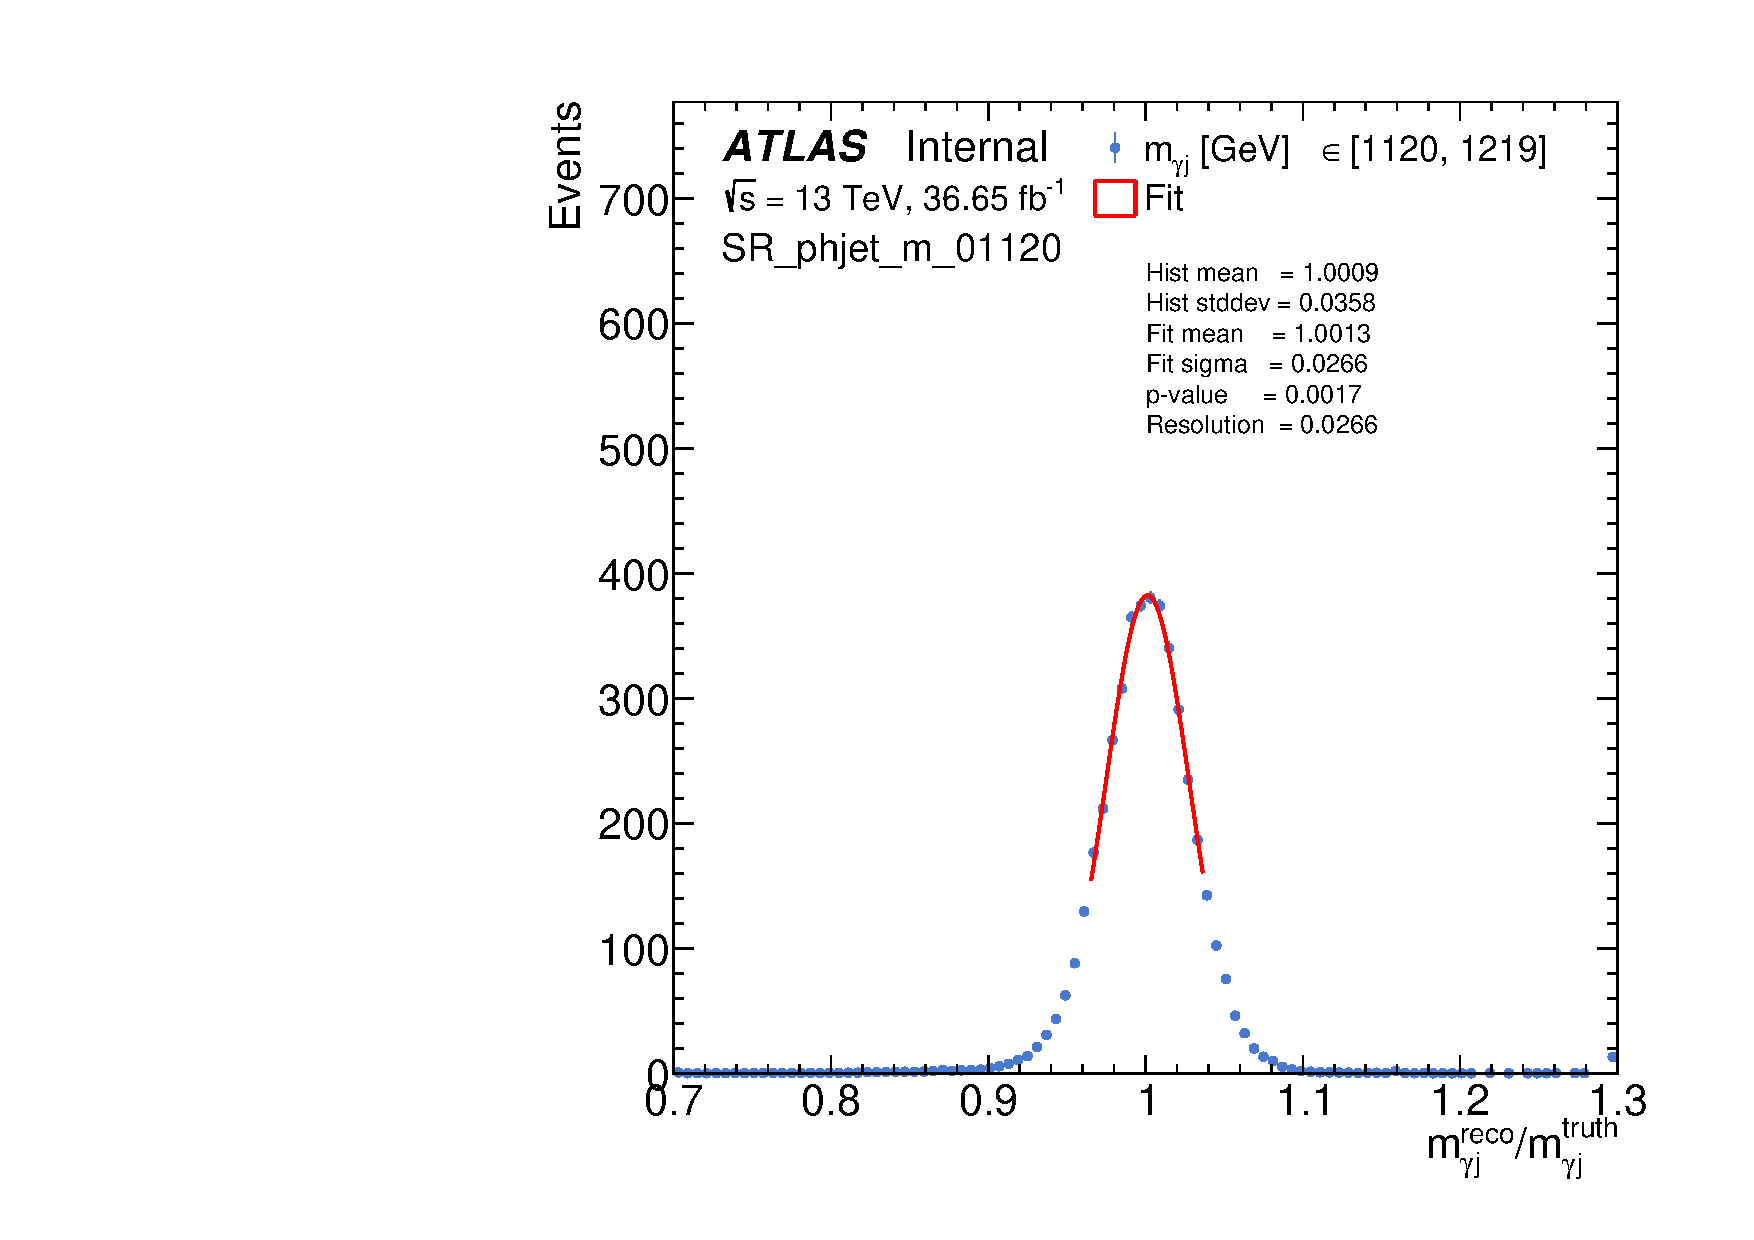
\includegraphics[width=0.32\linewidth]{5_resonances/results/myj_binning/distributions/can__phjet_m_over_phjet_truth_m__SR_phjet_m_01120}
    \hfill
    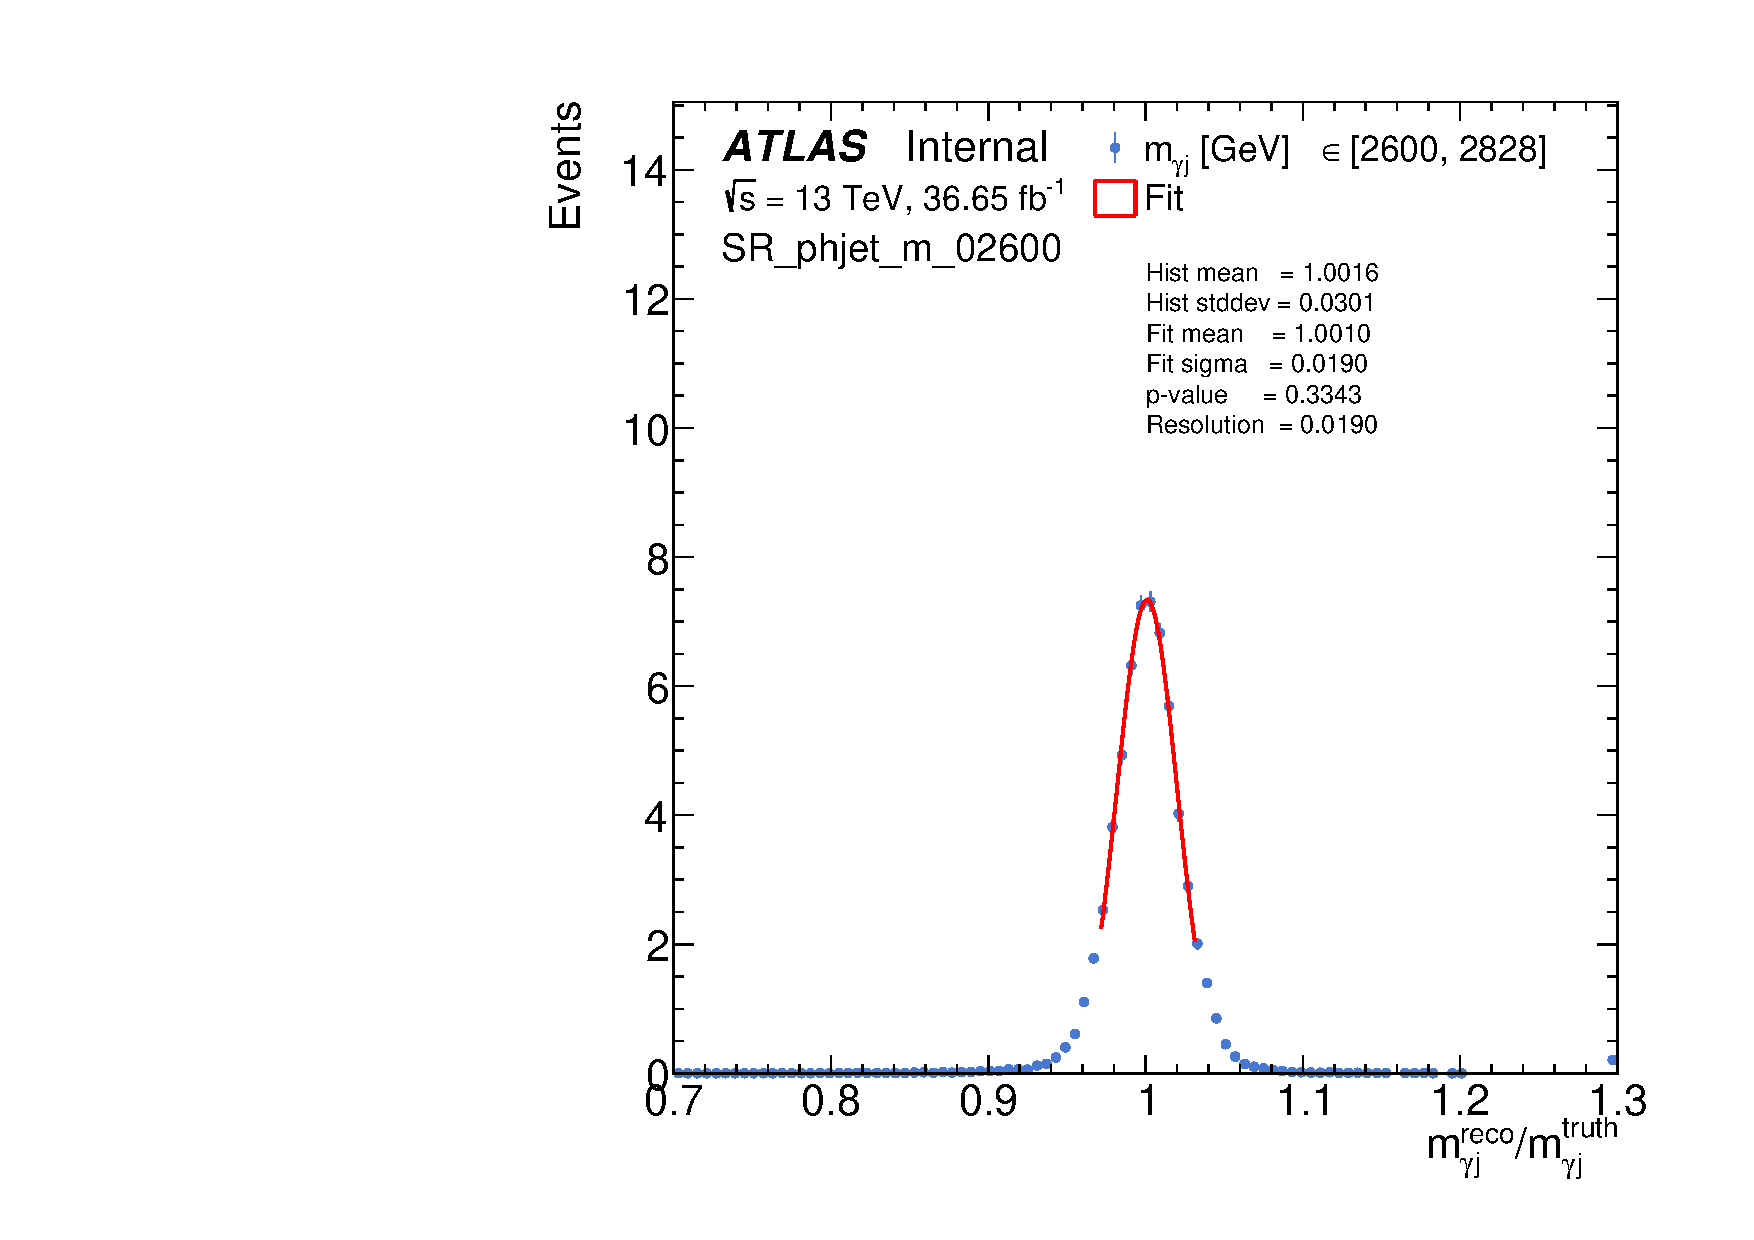
\includegraphics[width=0.32\linewidth]{5_resonances/results/myj_binning/distributions/can__phjet_m_over_phjet_truth_m__SR_phjet_m_02600}
    \hfill
    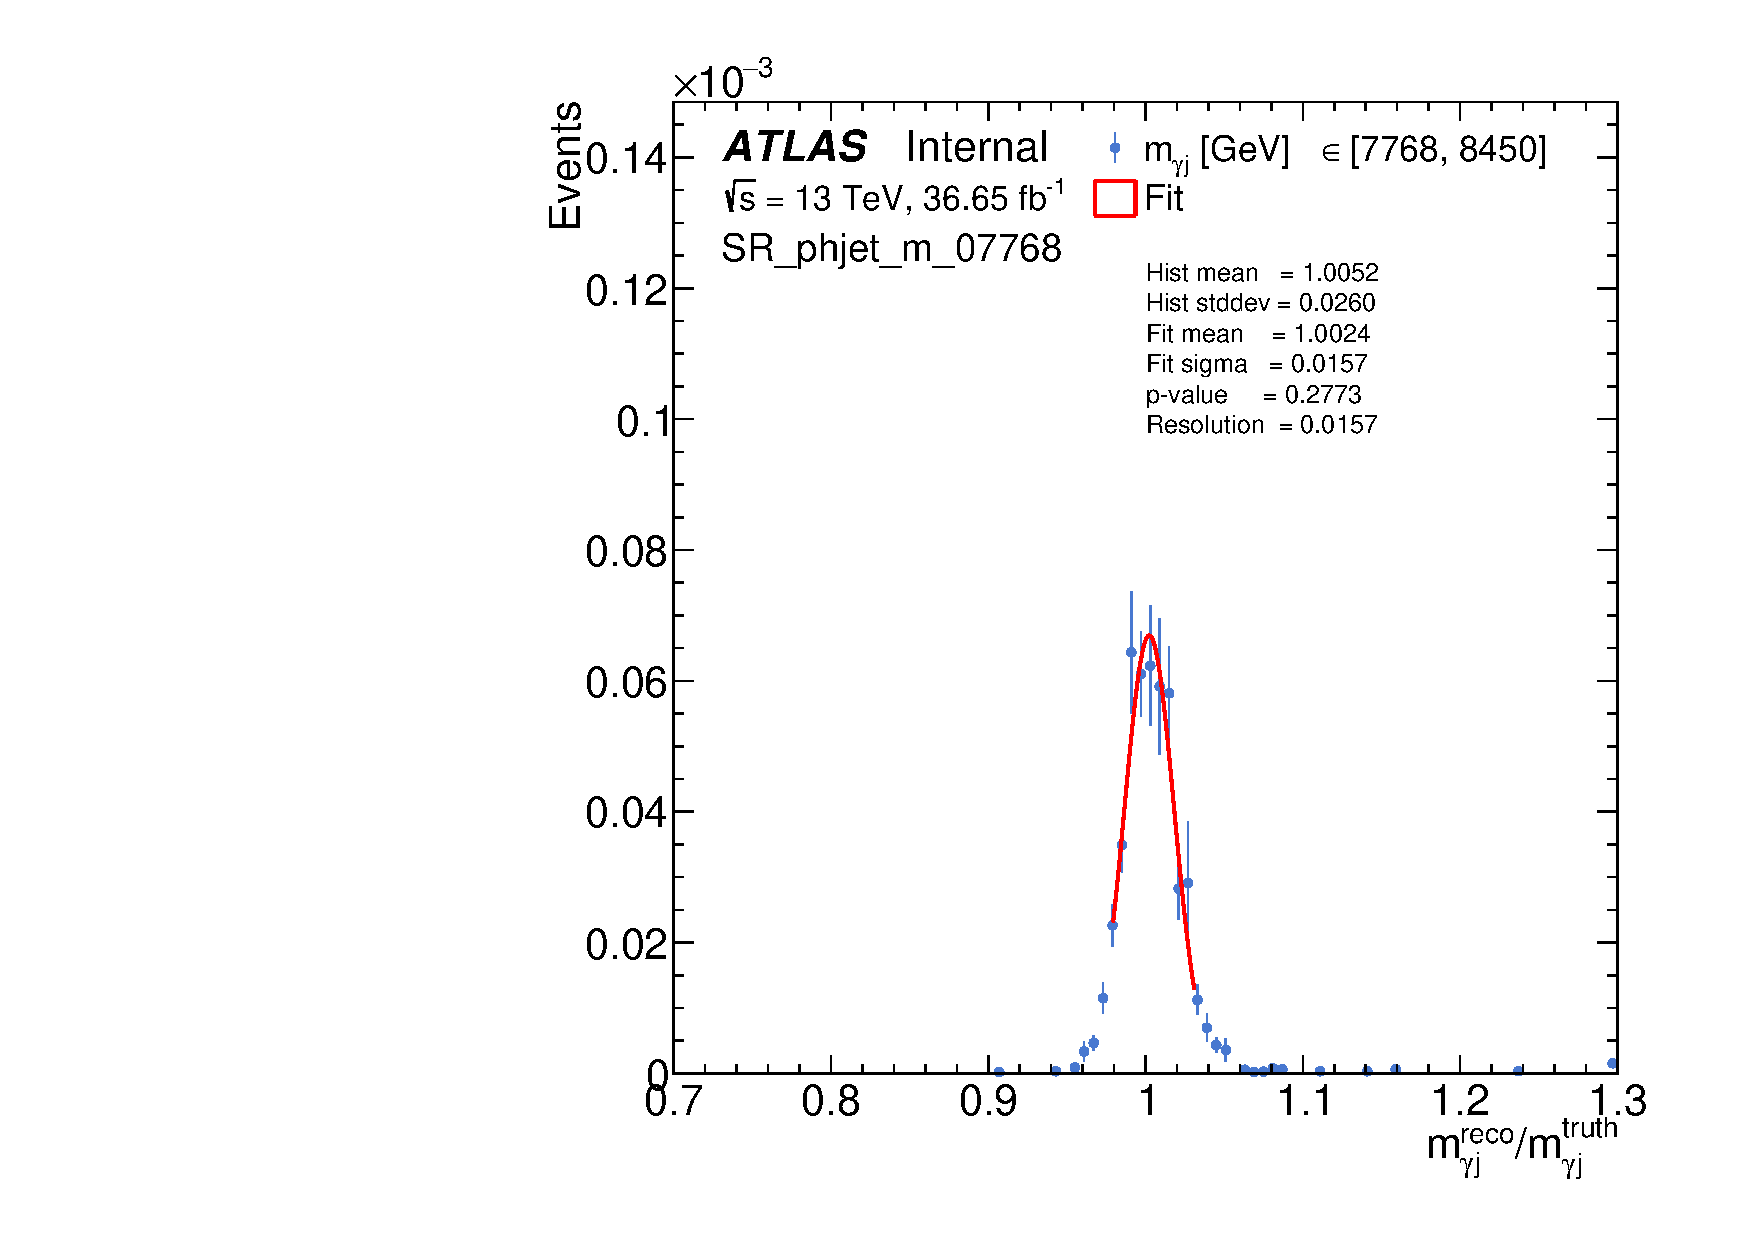
\includegraphics[width=0.32\linewidth]{5_resonances/results/myj_binning/distributions/can__phjet_m_over_phjet_truth_m__SR_phjet_m_07768}
    \caption{Ajustes seleccionados a las distribuciones de \(\myj^{reco} / \myj^{truth}\) necesarios para los estudios del binneado óptimo de \myj. Las distribuciones se muestran con los puntos azules y ajustes Gaussianos a ellas se muestran con la línea roja. Se muestra, en cada caso, el valor medio y el ancho de la distribución, así como también el valor medio y la desviación estándar de la Gaussiana ajustada.}
    \label{fig:results:obs:ratio_fits}
\end{figure}

\begin{figure}[ht!]
    \centering
    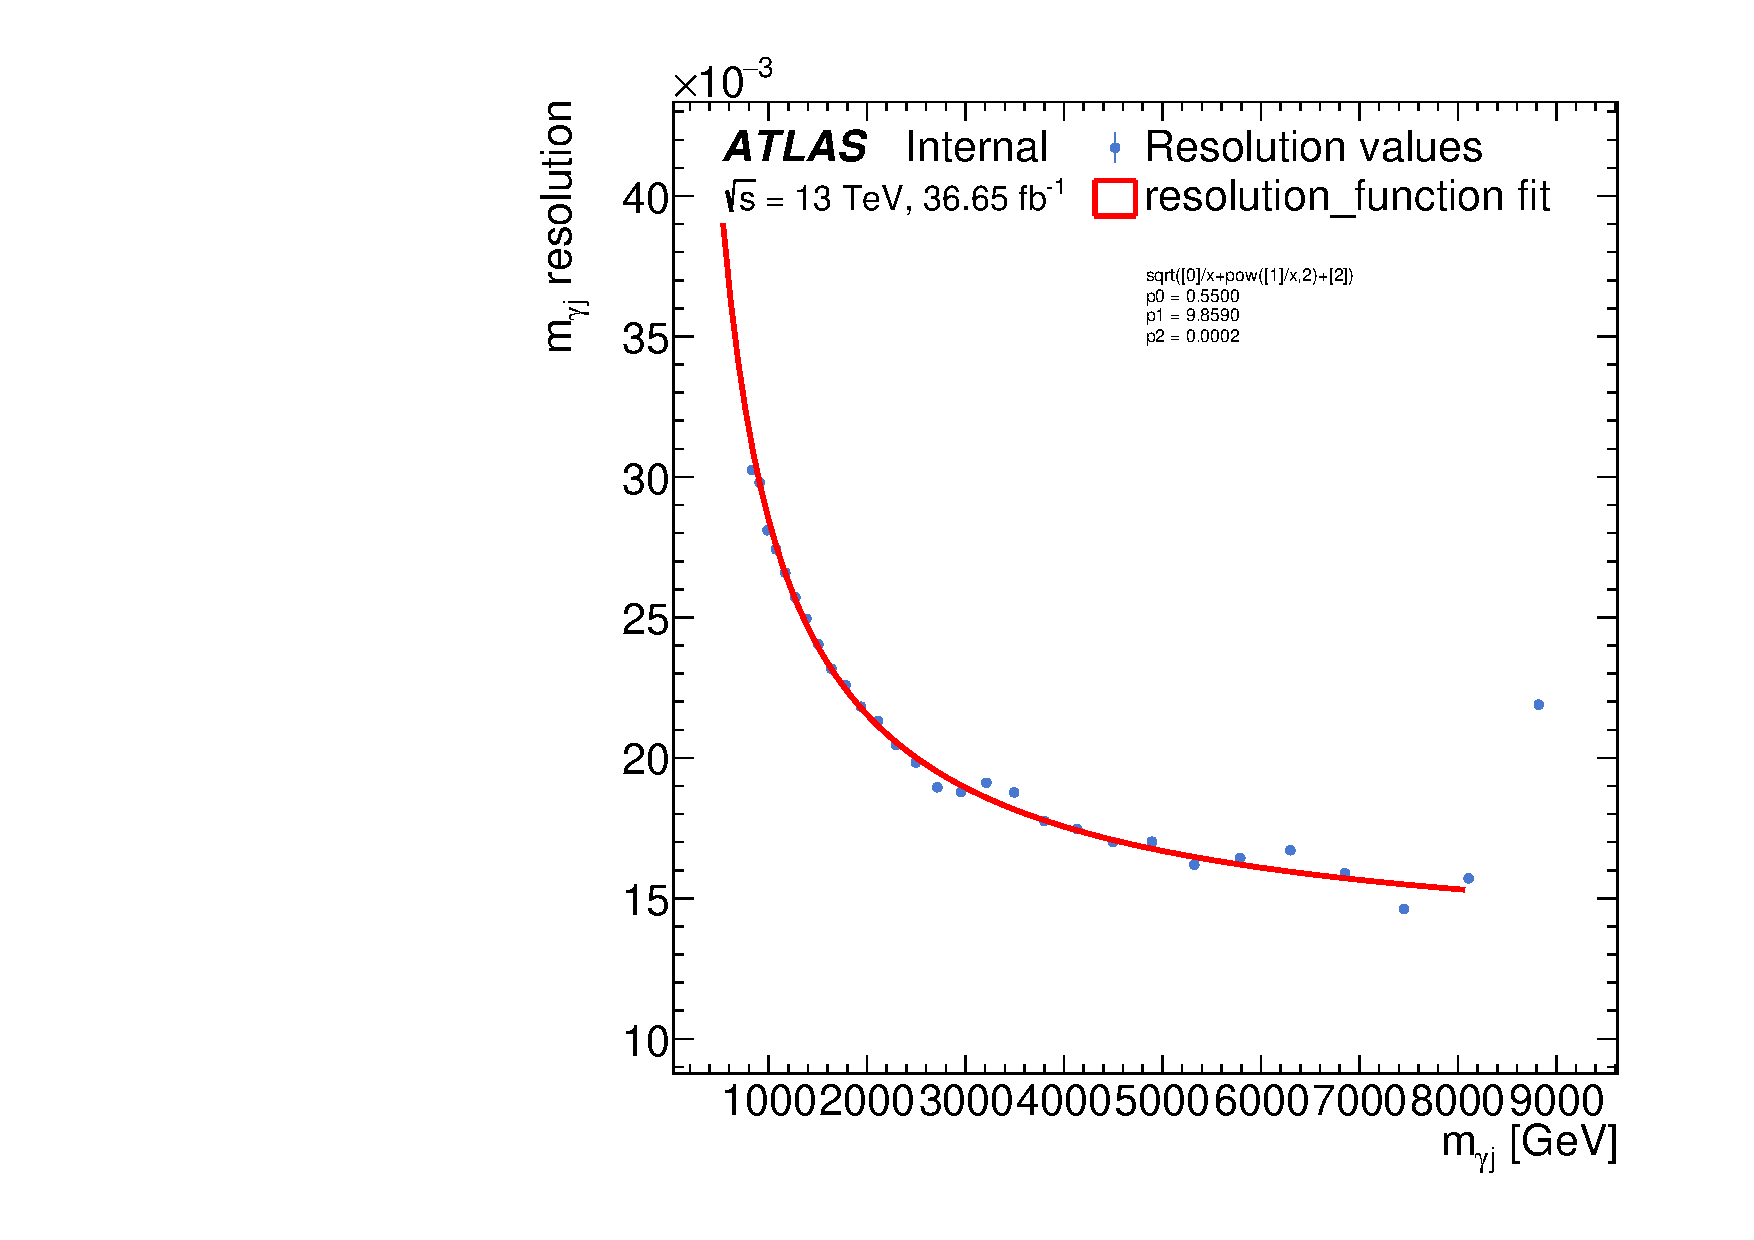
\includegraphics[width=0.7\linewidth]{5_resonances/results/myj_binning/resolution/can__phjet_m_over_phjet_truth_m_resolution__fit_resolution_function}
    \caption{Resolución del detector en \myj junto con su ajuste utilizando la función dada en la \Eqn{\ref{eq:results:obs:binning_resolution}}. Los parámetros ajustados de la función se muestran en la figura donde \(p_0 \equiv a\), \(p_1 \equiv b\) y \(p_2 \equiv c\). El ajuste se realiza excluyendo el último bin dado que no contaba con suficientes estadística.}
    \label{fig:results:obs:resolution_curve}
\end{figure}

% El binneado debe ser mayor que la resolución del detector. 
Para estimar la resolución del detector, se utilizan eventos de \gammajet simulados normalizados a la luminosidad del conjunto de datos 2015+2016. Como primer paso, los cocientes \(\myj^{reco} / \myj^{truth}\) se calculan en bines de \myj y para cada bin se ajusta una función Gaussiana \(g(\mu, \sigma)\) al cociente, como se muestra en la \Fig{\ref{fig:results:obs:ratio_fits}}. De los ajustes, el cociente entre el ancho y el valor medio de la Gaussiana, \(\sigma / \mu\), corresponde a la resolución. El conjunto resultante de valores de resolución se representa como una función de \myj y se le realiza un ajuste con una función de la forma
\begin{equation}
    \label{eq:results:obs:binning_resolution}
    \frac{\sigma}{\myj} = \sqrt{
        \frac{a}{\myj} +
        \left(\frac{b}{\myj}\right)^2 +
        c
    },
\end{equation}
que se muestran en la \Fig{\ref{fig:results:obs:resolution_curve}}. Por último, se calcula el binneado de \myj a partir de la función ajustada, empezando en \(500~\gev\) hasta \(10~\tev\), de forma iterativa hasta que el ancho del bin sea compatible con la resolución a un dado valor de \myj. Los anchos de los bines en función de \myj se muestra en la \Fig{\ref{fig:bkg_modeling:observable:results:binwidth}}, que muestra una naturaleza monotónicamente creciente como es de esperar. Finalmente, para validar que la resolución del binning concuerda con la del detector, en la \Fig{\ref{fig:bkg_modeling:observable:results:resolution_comparison}} se muestra una comparación entre ambas, de la que se observa una excelente concordancia.

\begin{figure}[ht!]
    \centering
    \begin{subfigure}[t]{0.49\linewidth}
        \centering
        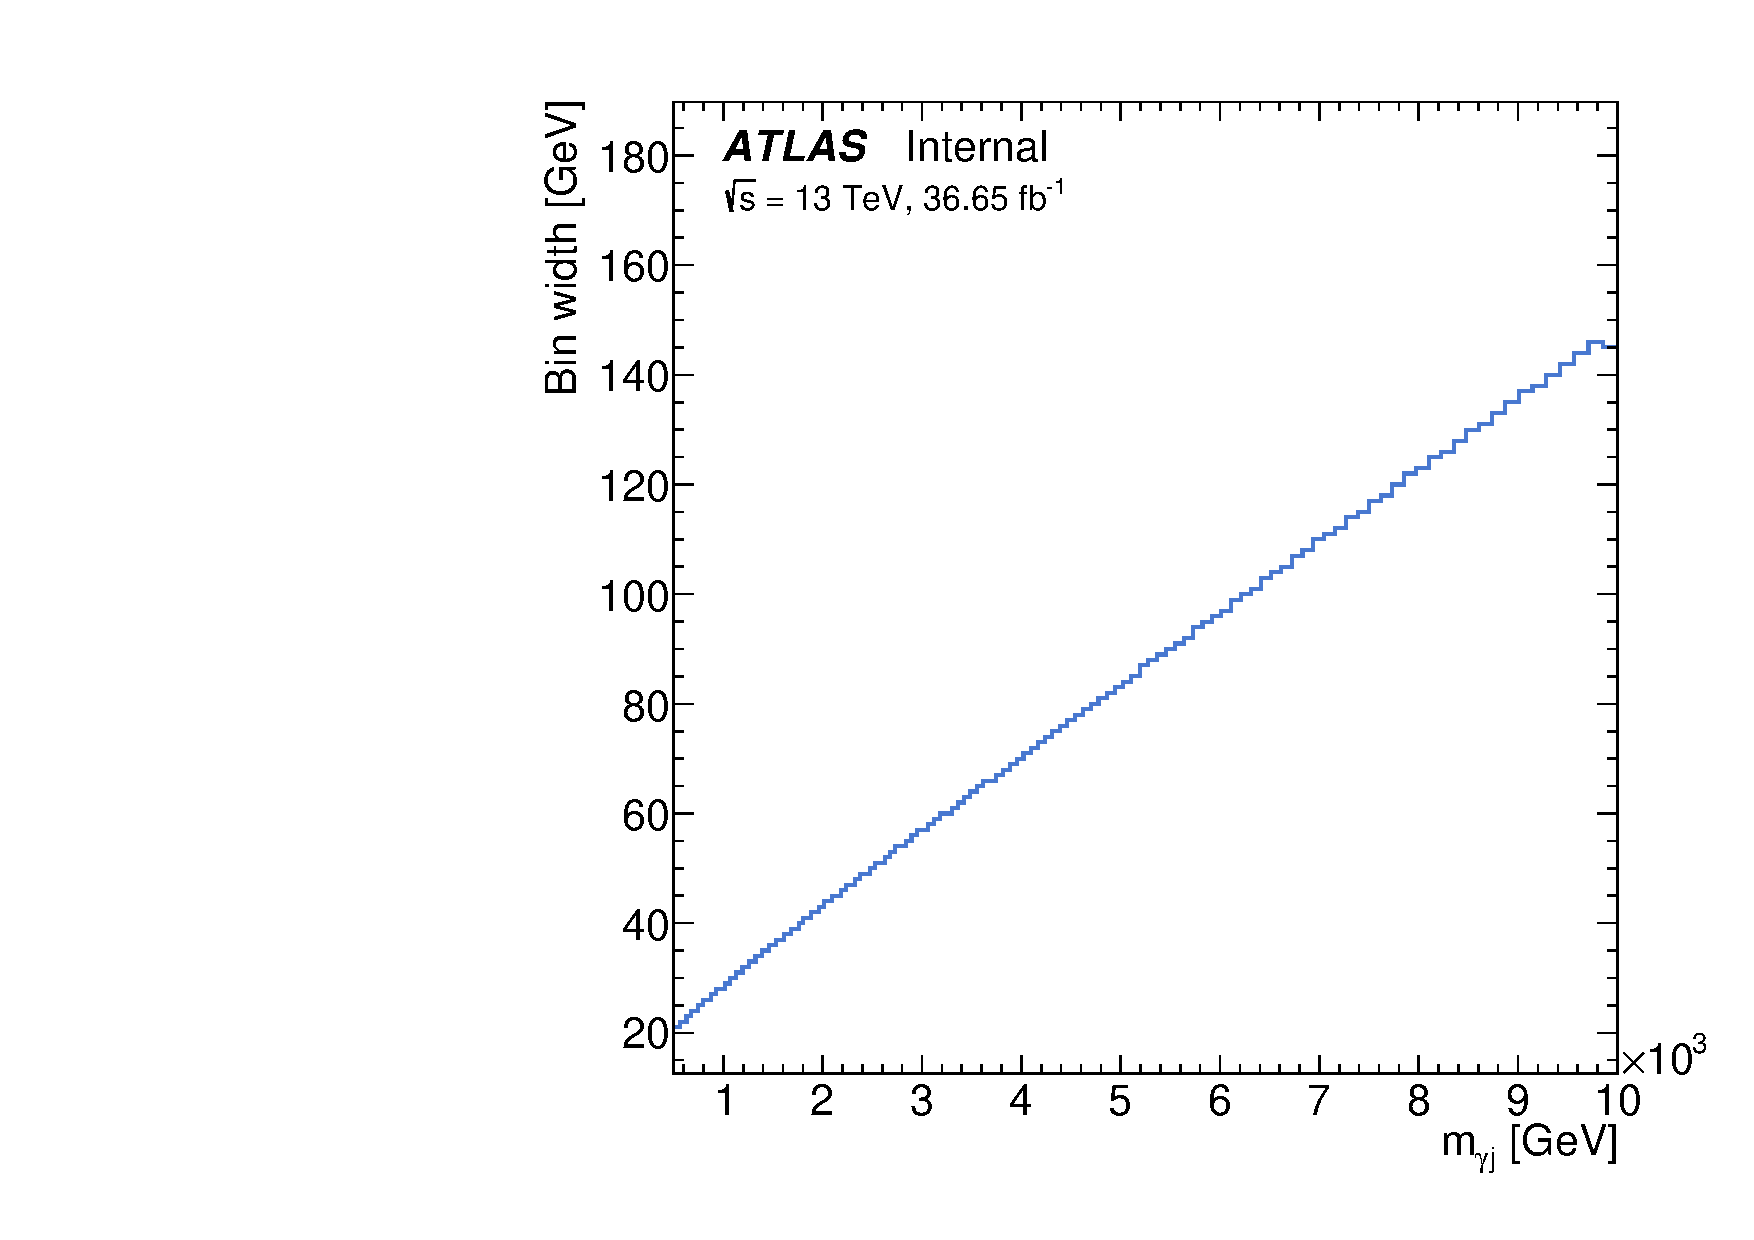
\includegraphics[width=\linewidth]{5_resonances/results/myj_binning/binning/can__SR__phjet_m_binwidth__2015_2016}
        \caption{Ancho de los bines en función de \myj.}
        \label{fig:bkg_modeling:observable:results:binwidth}
    \end{subfigure}
    \hfill
    \begin{subfigure}[t]{0.49\linewidth}
        \centering
        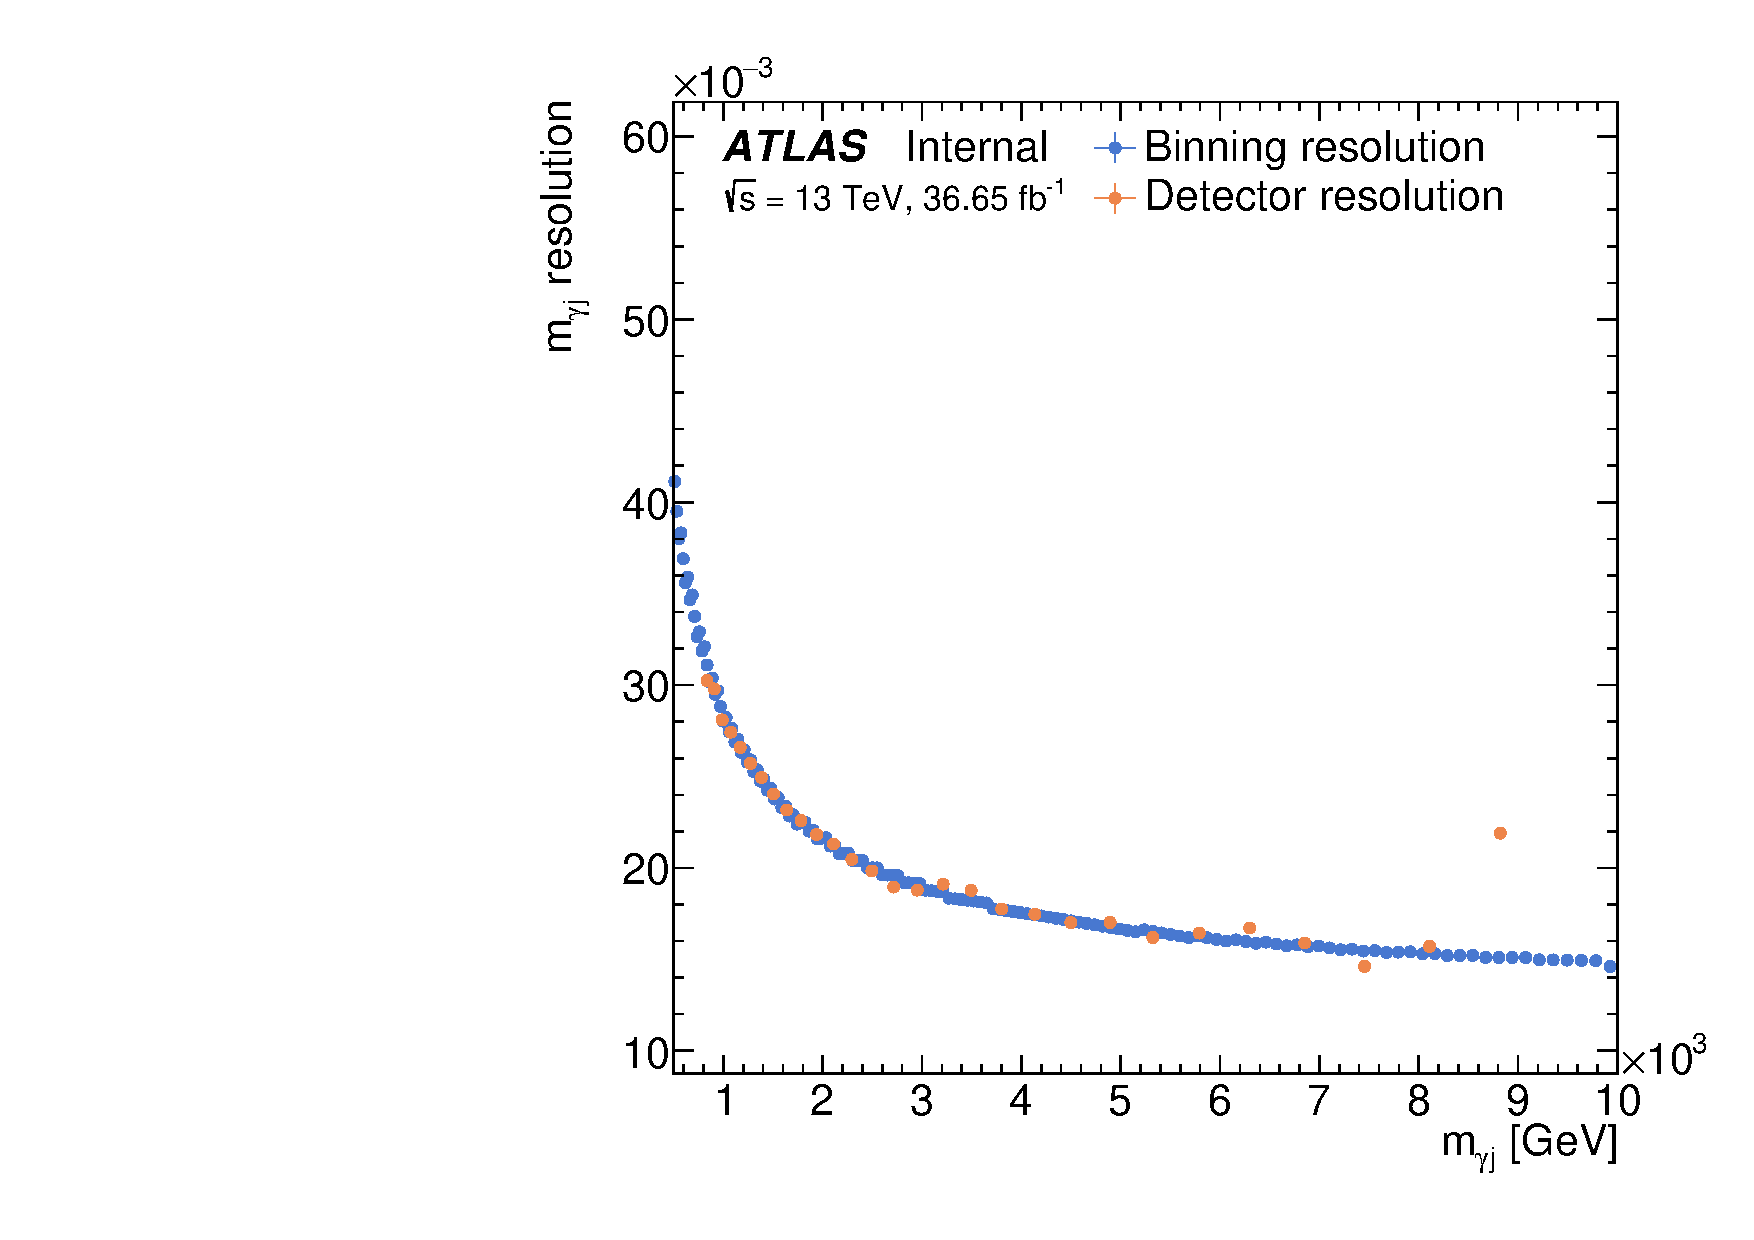
\includegraphics[width=\linewidth]{5_resonances/results/myj_binning/binning/can__SR__phjet_m_binresolution__2015_2016}
        \caption{Resolución del detector y la obtenida a partir del binneado.}
        \label{fig:bkg_modeling:observable:results:resolution_comparison}
    \end{subfigure}
    \caption{Resultados de la optimización del binneado de \myj mostrando los anchos de los bines como función de \myj (izquierda) y la comparación entre las resoluciones del detector y la obtenida del binneado (derecha).}
    \label{fig:bkg_modeling:observable:results}
\end{figure}



























\section{Resultados}
\label{sec:results:results}

Una vez definidas las estrategias de ajuste para cada una de las regiones de señal y modelos de señal considerados (véase la \Tab{\ref{tab:bkg:modeling:strategy_modeling:summary}}), se aplican ahora los ajustes a las distribuciones de \myj observados en los datos. Se estudian dos tipos de interpretaciones:
\begin{itemize}
    \item \textbf{Ajustes \Acf{BO}}: Se realiza un ajuste de \ac{BO} a los datos en cada una de las regiones de señal para comprobar la compatibilidad de los datos con un espectro de masas que decae suavemente. En caso de que se encuentre algún exceso, se cuantifica en virtud del algoritmo \bh comentado anteriormente.
    \item \textbf{Ajustes \Acf{SB}}: Se estudia la compatibilidad de los datos con tres modelos de señal diferentes. Uno de los modelos corresponde a formas gaussianas genéricas que permiten interpretar los resultados de forma más general. Los otros dos modelos teóricos estudiados corresponden a los modelos \acp{QBH} y \acp{EQ}, donde sus formas de resonancia son diferentes entre ellos y también para diferentes parámetros de las teorías. En caso de que no se encuentre un exceso significativo en la interpretación de \ac{BO}, se derivan límites de exclusión en los valores de los parámetros de estas teorías.
\end{itemize}







\subsection{Resultados de ajuste sólo-fondo}
\label{subsec:results:results:bkgonly}

El ajuste de \ac{BO} permite realizar una interpretación de la distribución de masas invariante sin ninguna suposición sobre la señal potencial, aparte de que se encuentre algún efecto localizado. Sin embargo, la consistencia entre el espectro \myj observado con un fondo del \ac{SM} suavemente decreciente no puede cuantificarse únicamente con el valor \(p(\chisq)\). Esta medida no proporciona la sensibilidad óptima a una resonancia localizada ya que considera todos los bines de \myj simultáneamente e independientemente unos de otros. Por otro lado, una resonancia real probablemente daría lugar a un exceso correlacionado en uno o varios bines de \myj adyacentes y aquí es cuando entra en juego el algoritmo \bh.

\begin{figure}[ht!]
    \centering
    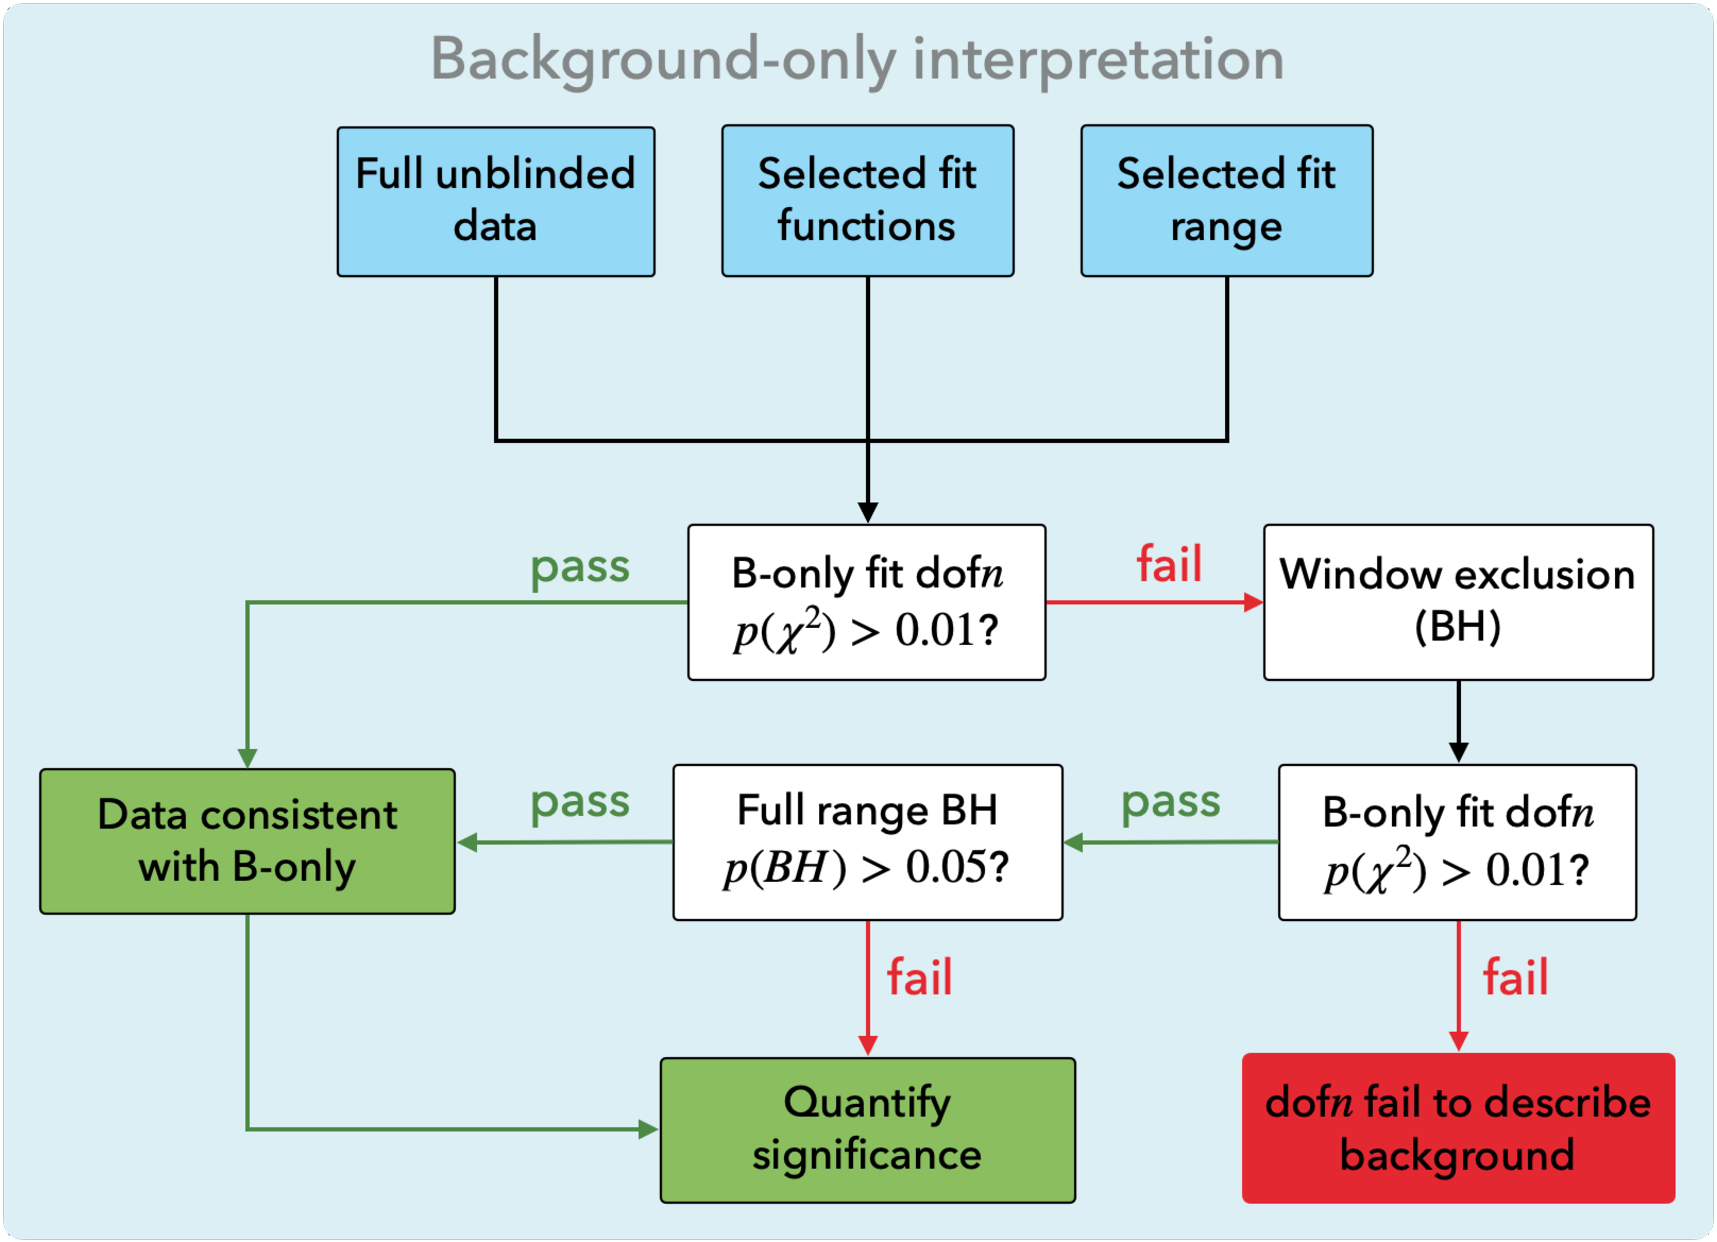
\includegraphics[width=0.7\linewidth]{5_resonances/results/bkgonly/unblind_strategy3_bo}
    \caption{Esquema del procedimiento utilizando para los ajustes de \ac{BO} a los datos.}
    \label{fig:results:results:bkgonly:strat}
\end{figure}

El proceso de ajuste de \ac{BO} se muestra en la \Fig{\ref{fig:results:results:bkgonly:strat}}. Para cada región de señal, el primer paso es realizar un ajuste de \ac{BO} al espectro de masas. Si el \(p(\chisq)\) de este ajuste supera un umbral de 0.01, la hipótesis de \ac{BO} logra describir los datos y se ejecuta el algoritmo de \bh para identificar la desviación más significativa y asignarle un valor-\(p\). Por otro lado, si \(p(\chisq) < 0.01\), esto puede indicar que el ajuste no es capaz de describir globalmente el espectro de datos o que hay una o varias desviaciones localizadas. Para comprobar este último caso, se ejecuta el algoritmo de \bh para identificar la desviación más significativa. A continuación, se remueve (o enmascara) esta región y se repite el ajuste de \ac{BO} y se vuelve a comprobar el valor \(p(\chisq)\). Si no supera el umbral, un único efecto local no puede explicar el mal ajuste y no se puede dar una interpretación clara del espectro observado. Si, por el contrario, se supera el umbral, significa que, efectivamente, el efecto local impedía un buen ajuste. Se vuelve a ejecutar el \bh y se asigna un \pval a esta desviación más significativa. Un \pval mayor que 0.05 se interpreta entonces como que no se ha descubierto ninguna resonancia significativa. Si, por el contrario, no se supera este umbral, se supone un efecto local y se evalúa la importancia de la señal hipotética.



\subsubsection{Resultados}

\begin{figure}[ht!]
    \centering
    \begin{subfigure}[h]{0.49\linewidth}
        \centering
        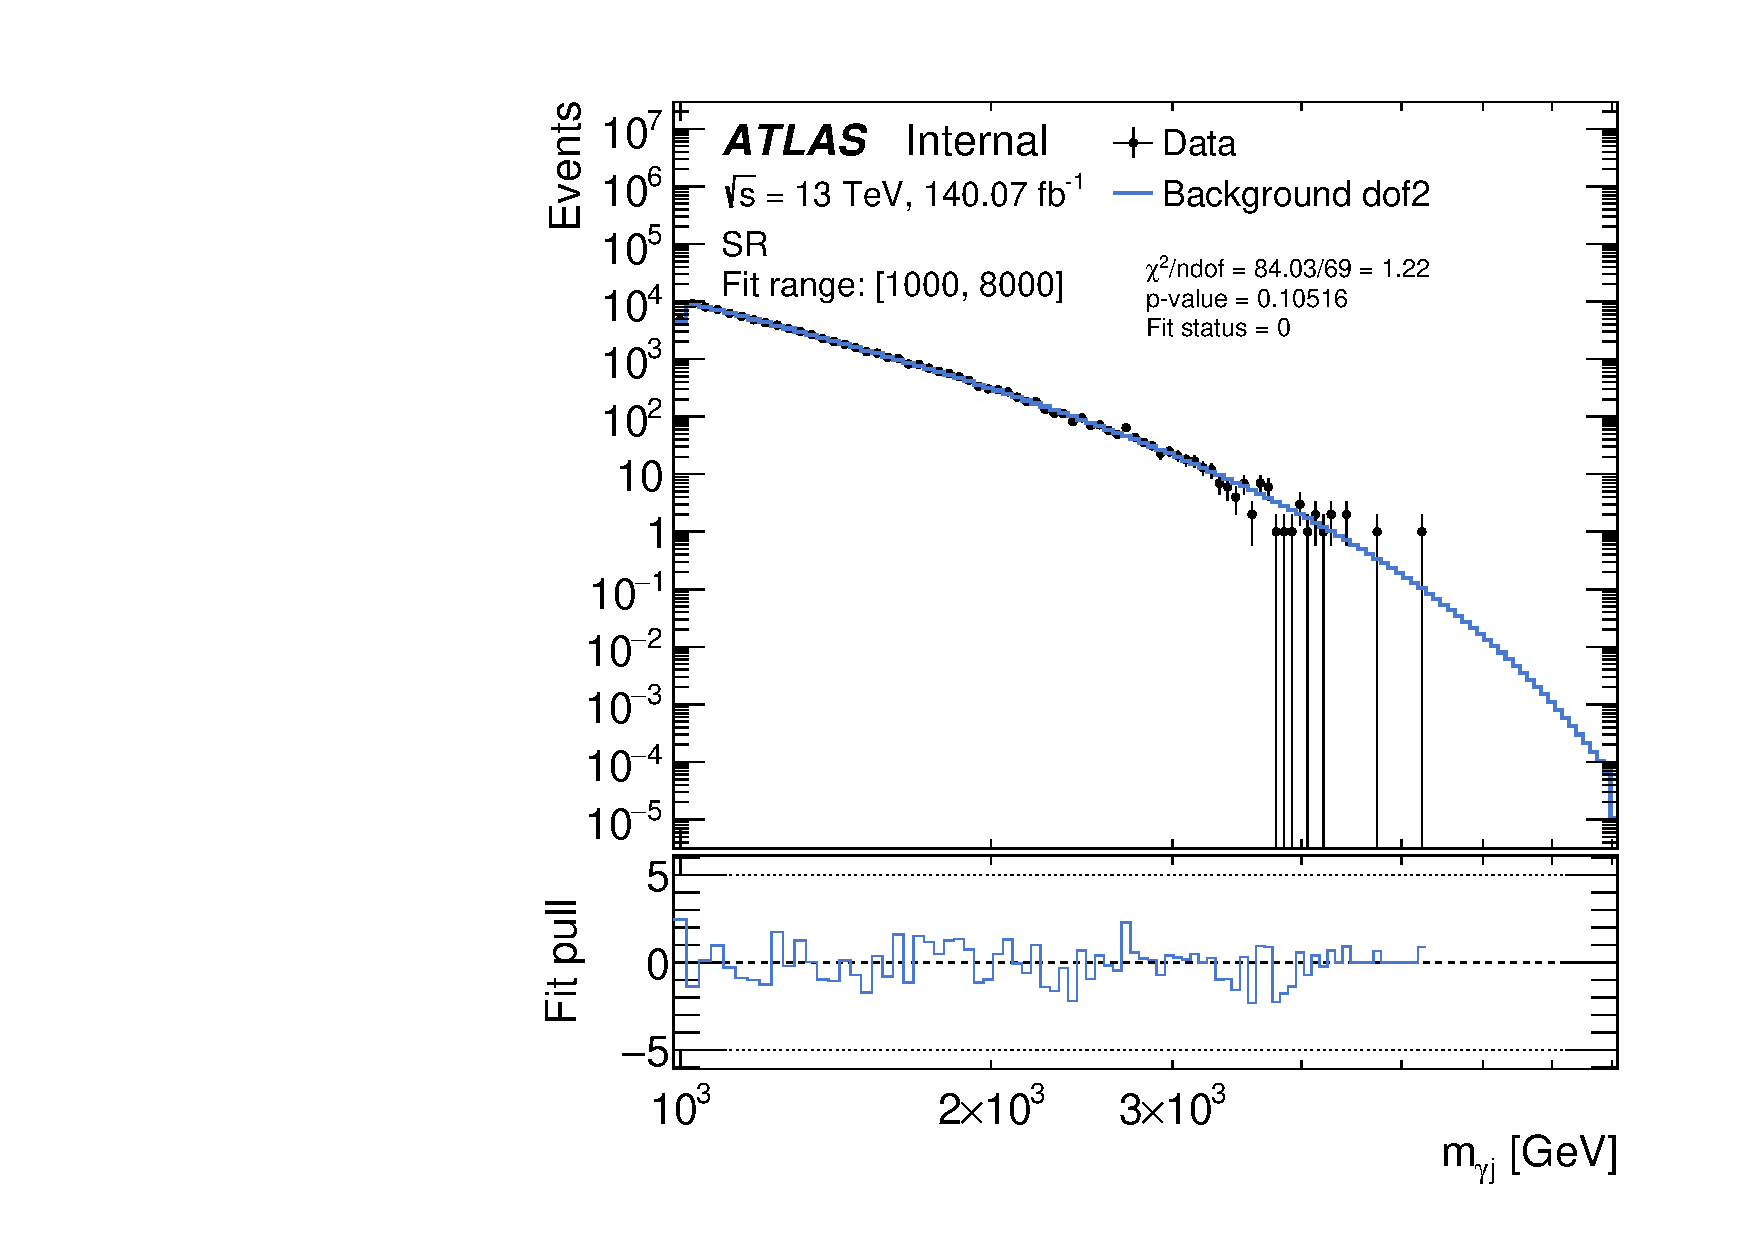
\includegraphics[width=\linewidth]{5_resonances/results/bkgonly/SR/dof2__range_1000_8000/plots/can__bkgonlyfit__asimov__data__SR__dof2__range_1000_8000}
        \caption{SR}
        \label{fig:results:results:bkgonly:fits:SR}
    \end{subfigure}
    \hfill
    \begin{subfigure}[h]{0.49\linewidth}
        \centering
        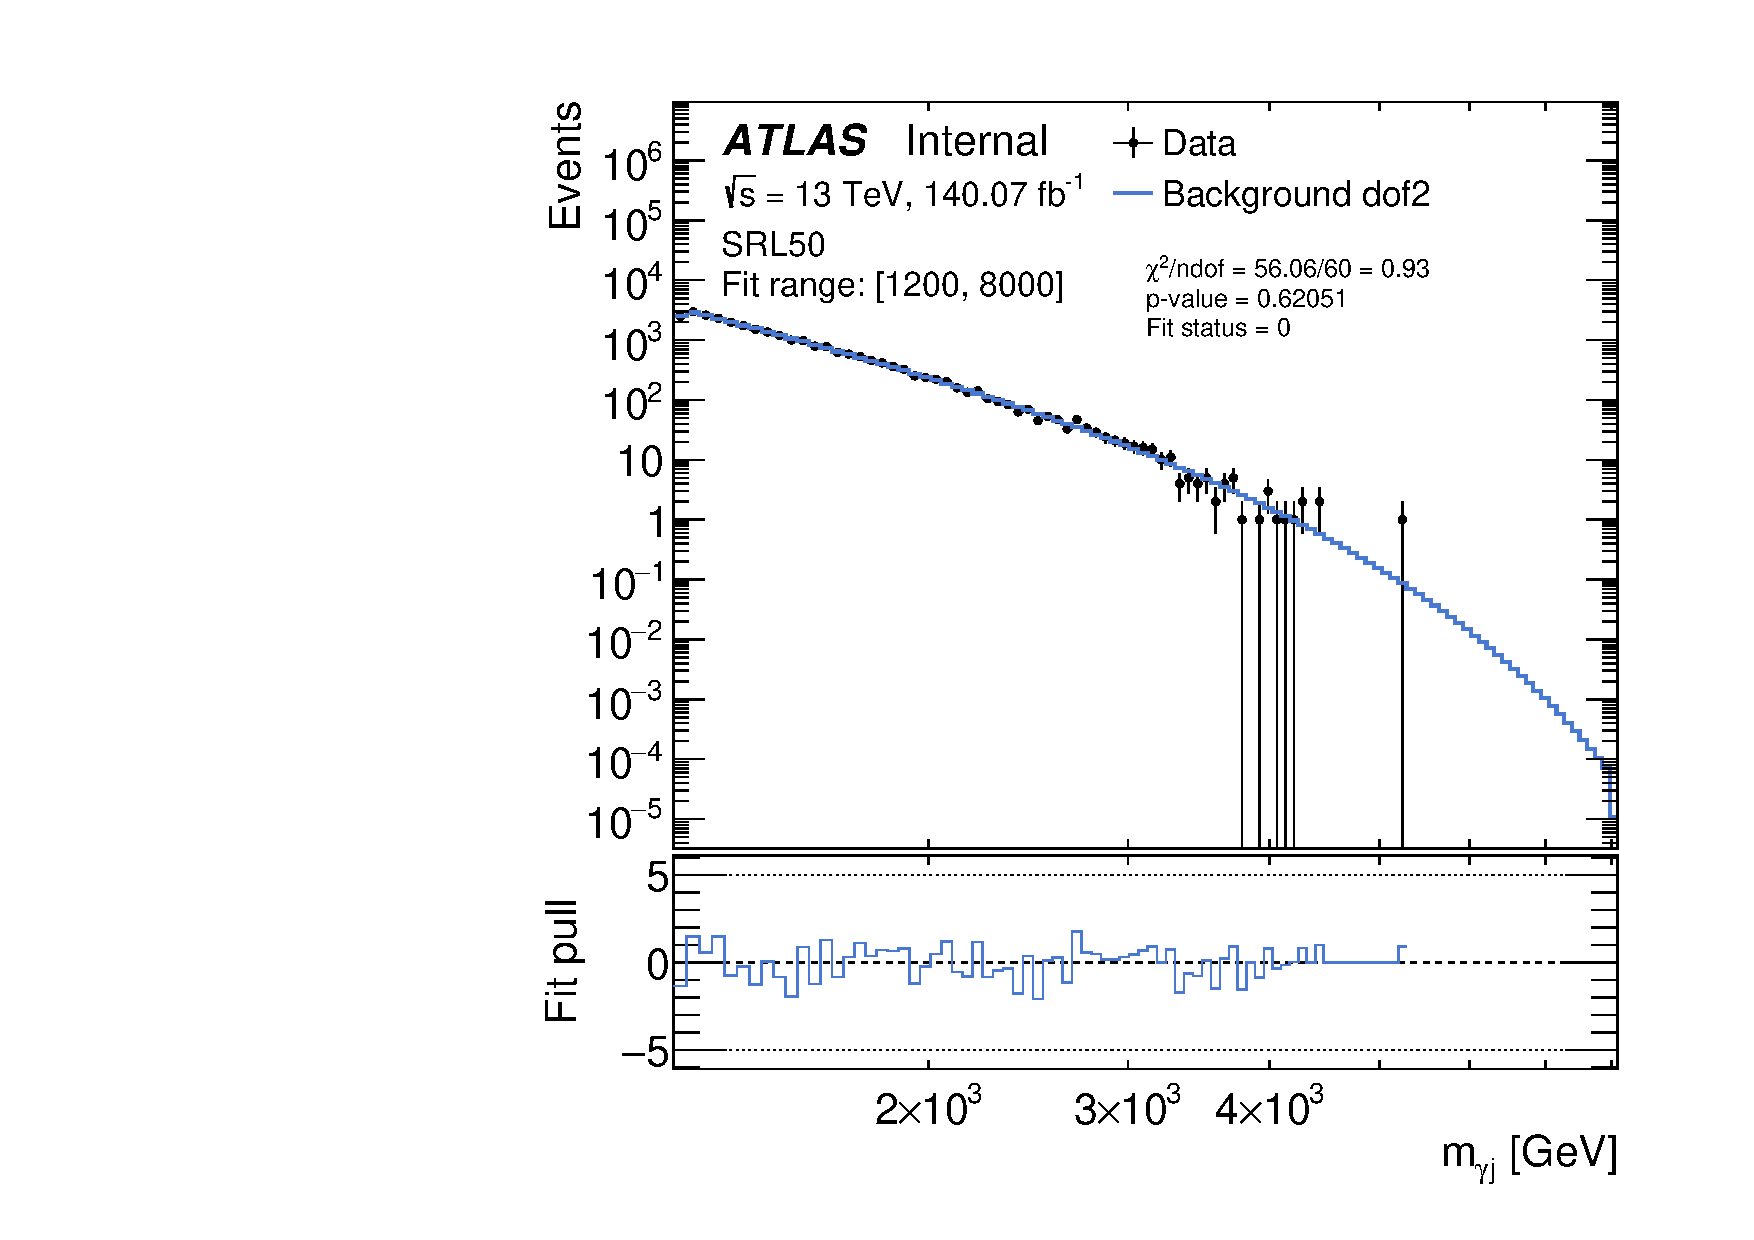
\includegraphics[width=\linewidth]{5_resonances/results/bkgonly/SRL50/dof2__range_1200_8000/plots/can__bkgonlyfit__asimov__data__SRL50__dof2__range_1200_8000}
        \caption{SRL}
        \label{fig:results:results:bkgonly:fits:SRL50}
    \end{subfigure}\\
    \begin{subfigure}[h]{0.49\linewidth}
        \centering
        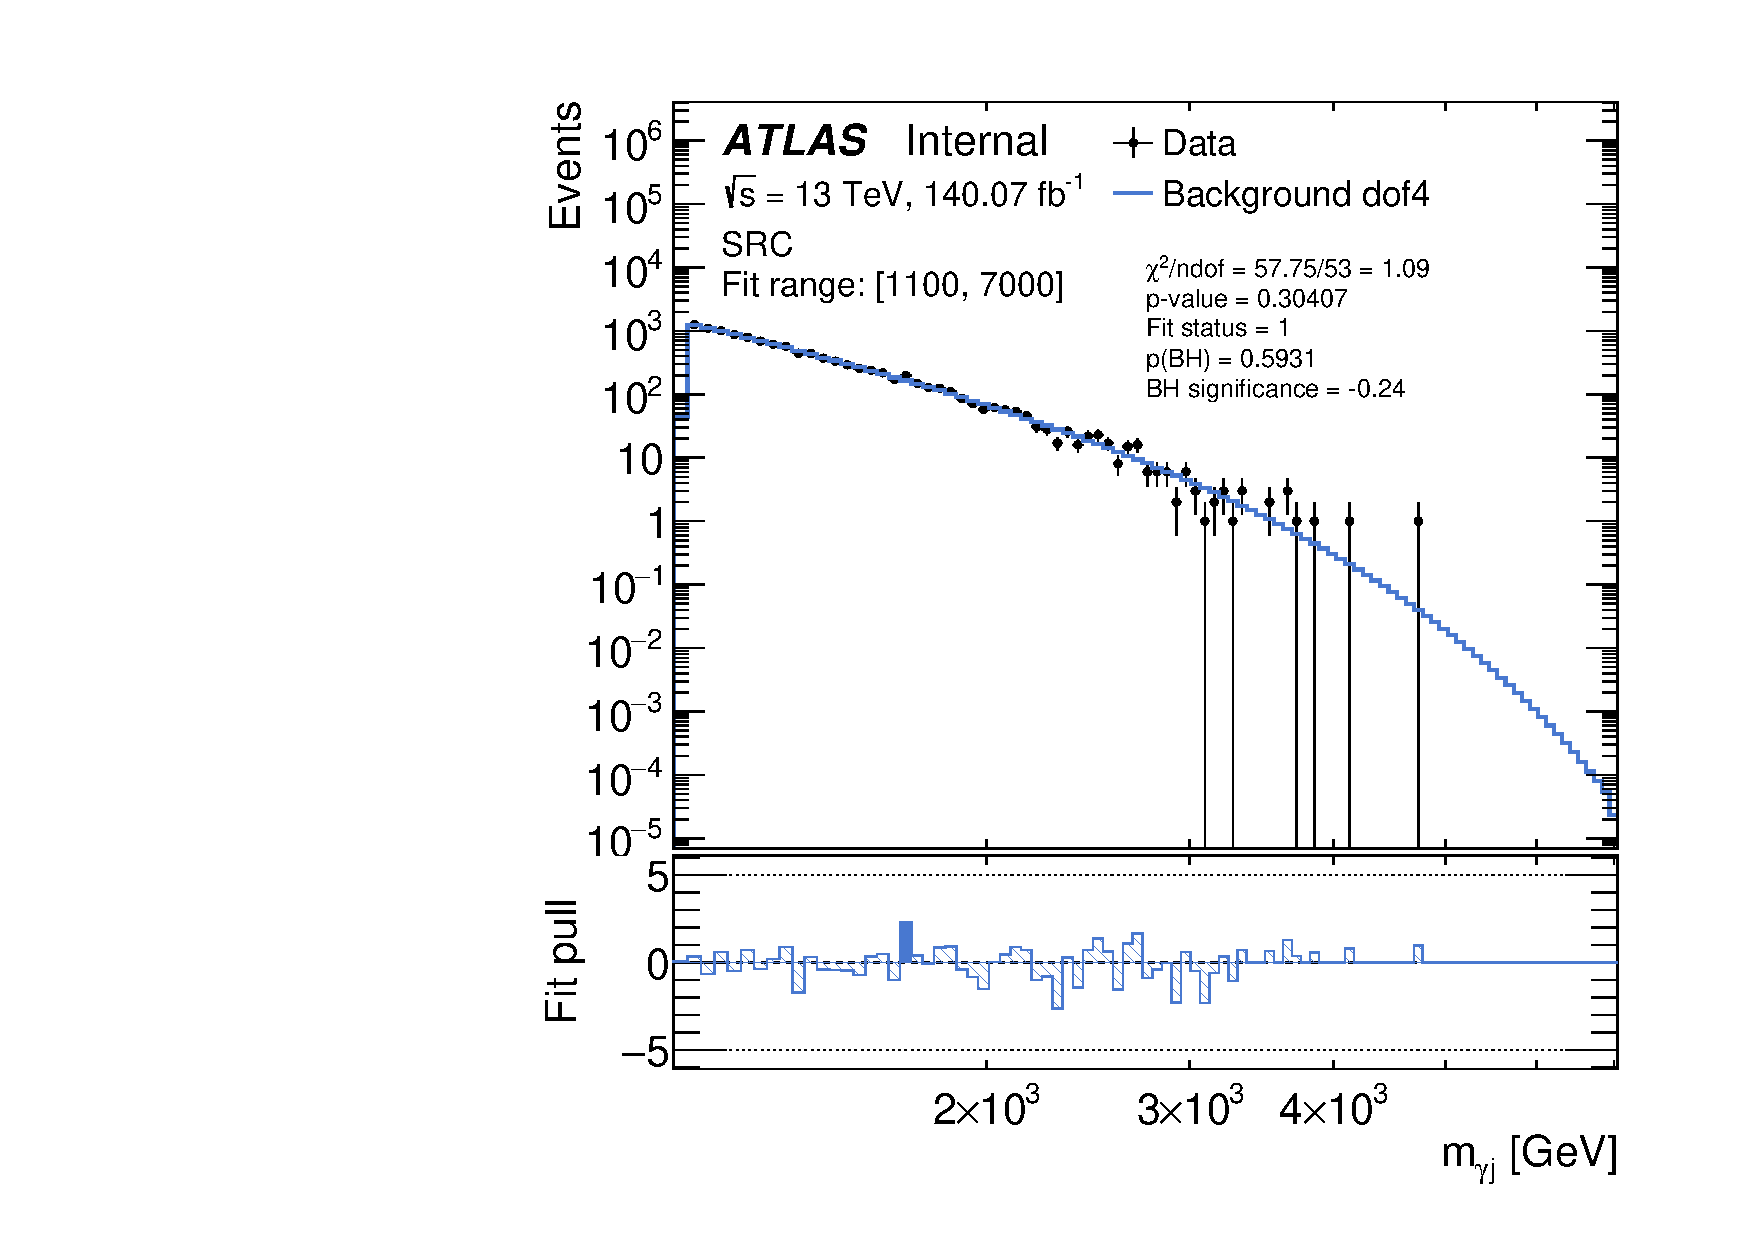
\includegraphics[width=\linewidth]{5_resonances/results/bkgonly/SRC50/dof4__range_1100_7000/plots/can__bkgonlyfit__asimov__data__SRC50__dof4__range_1100_7000}
        \caption{SRC}
        \label{fig:results:results:bkgonly:fits:SRC}
    \end{subfigure}
    \hfill
    \begin{subfigure}[h]{0.49\linewidth}
        \centering
        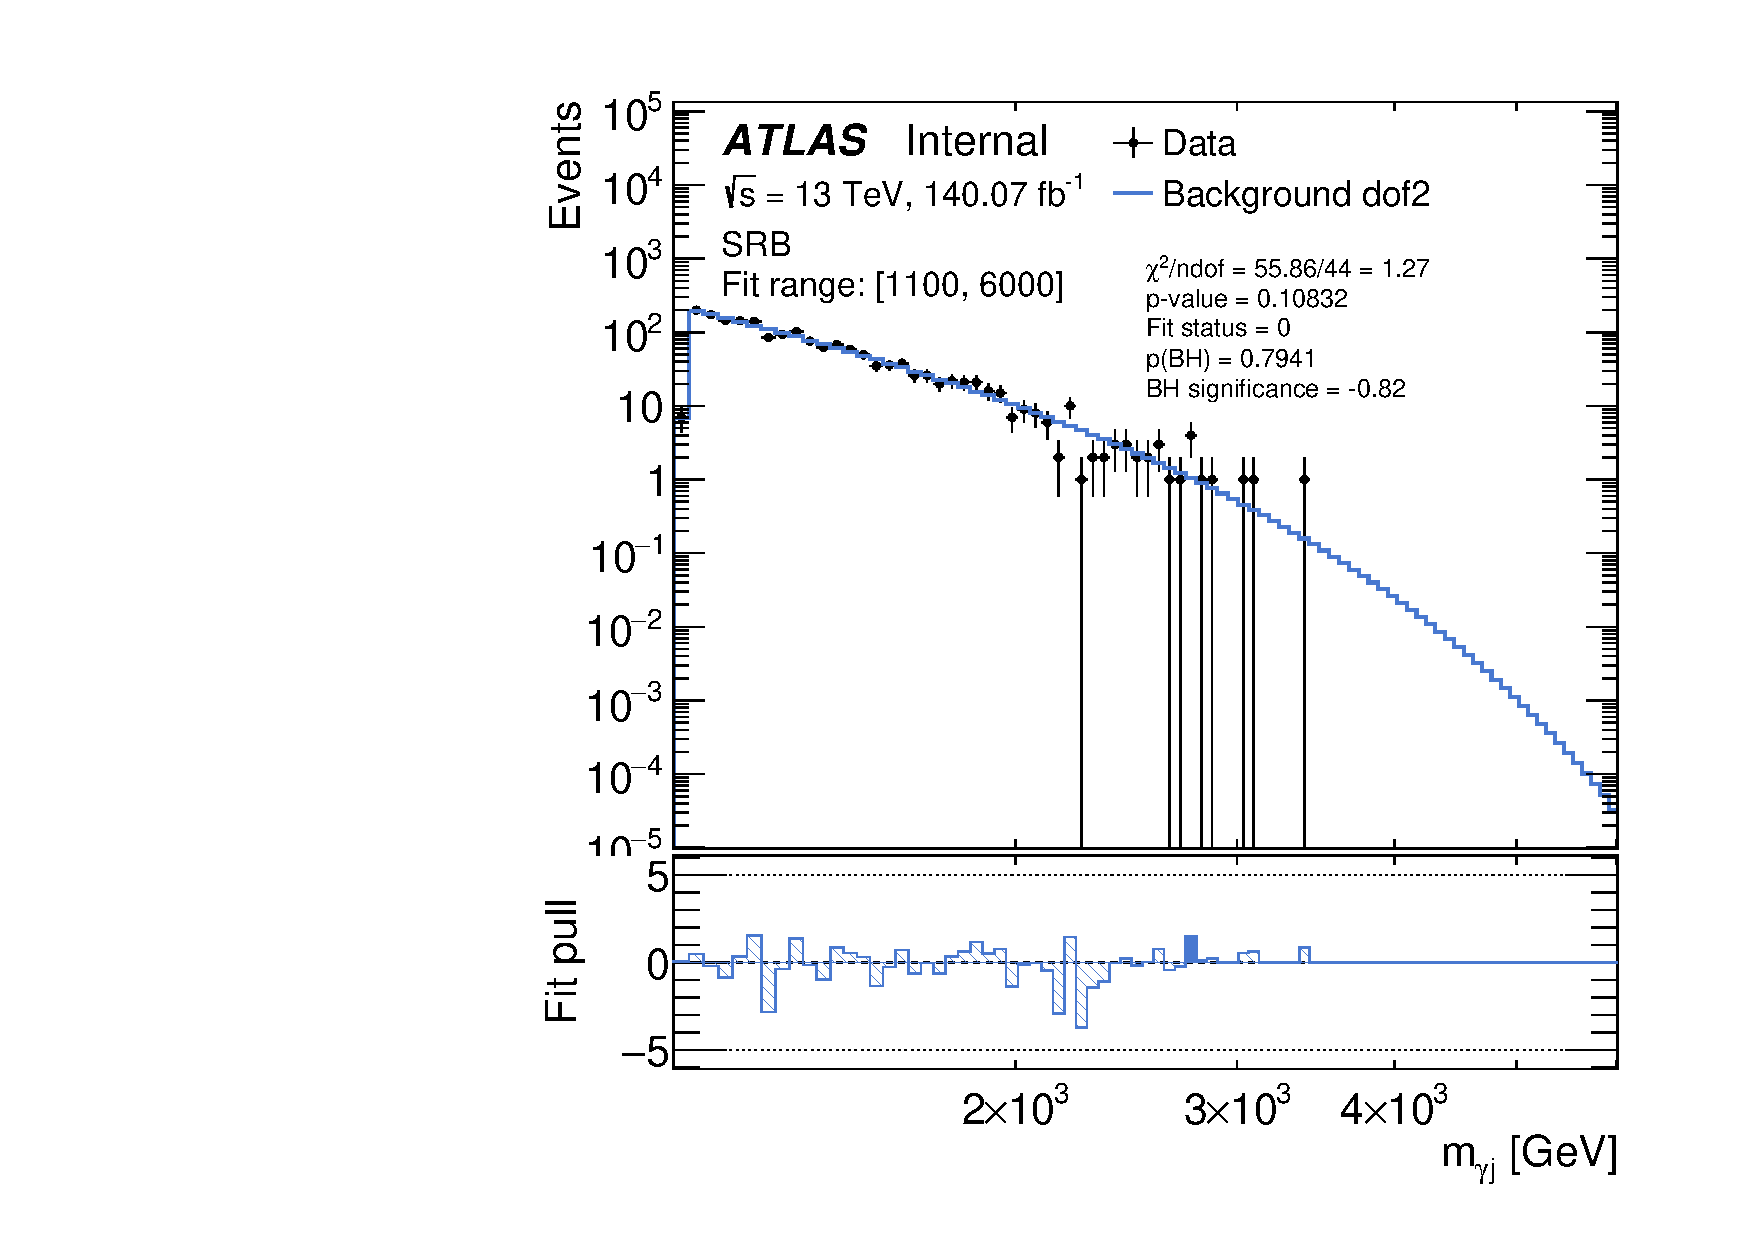
\includegraphics[width=\linewidth]{5_resonances/results/bkgonly/SRB/dof2__range_1100_6000/plots/can__bkgonlyfit__asimov__data__SRB__dof2__range_1100_6000}
        \caption{SRB}
        \label{fig:results:results:bkgonly:fits:SRB}
    \end{subfigure}
    \caption{Ajustes de \ac{BO} a los datos completos del Run-2 en las cuatro regiones consideradas en el análisis. Las distribuciones de los datos se muestran en el panel superior, donde los datos son representados por los puntos negros, mientras que la línea azul representa la función que describe al fondo del \ac{SM}. En los paneles inferiores se muestran los residuos normalizados (o pull) por las incertezas estadísticas de los datos. Los bines del panel inferior rellenos con el color azul denotan el exceso más significativo encontrado por el algoritmo de \bh. Además, el \chisq y valor \(p\) del ajuste se muestran en cada figura junto con el valor \(p \left(\text{BH}\right)\) y la significancia del algoritmo \bh.}
    \label{fig:results:results:bkgonly:fits}
\end{figure}

Los ajustes resultantes en cada región de señal se muestran en la \Fig{\ref{fig:results:results:bkgonly:fits}}. Se puede observar que no se encuentra ningún exceso significativo en ninguna de las regiones, como lo indican los valores \(p\) mostrados para cada caso. En las figuras, el panel inferior muestra los residuos normalizados del ajuste donde se pueden identificar más fácilmente las diferencias entre los datos y la hipótesis de \ac{BO}. Las principales diferencias observadas entre la estimación de fondo y los datos reales son las fluctuaciones hacia abajo de los datos, especialmente en la región SRB en \(\sim 2100~\gev\). Este tipo de fluctuaciones hacen que la calidad del ajuste disminuya, aunque no drásticamente. Principalmente, estos casos se ven en las regiones SR y SRB que coincide con los casos en los que los valores \(p\) son \(\sim 10\%\).
Se puede notar que hay diversos casos en los que hay bines en las distribuciones que presentan diferencias de hasta \(+2\sigma\). Estas desviaciones serán identificadas a continuación empleando el método de \bh.


Teniendo en cuenta que los valores \(p(\chisq)\) en los ajustes de \ac{BO} no están por debajo del umbral del \(1\%\), es decir, que no existe ninguna diferencia significativa entre el modelo de fondo y los datos, se ejecuta el algoritmo dedicado \bh para identificar dónde se encuentra la desviación más significativa. Además, la desviación se cuantifica en términos del valor \(p\) de \bh, \(p \left(\text{BH}\right)\), calculado como se indica en la \Eqn{\ref{eq:strategy:stat_treatment:bh:bh_pval}}. Esto se logra calculando un valor \(p\) local comparando todas las ventanas (conjuntos de bines adyacentes) posibles dentro del rango del ajuste con los datos. Aquella ventana en donde el valor \(p\) local sea menor, se identifica como la ventana más signficativa y se muestra en la \Fig{\ref{fig:results:results:bkgonly:fits}} con bines rellenos en el pull mostrado en el panel inferior. Asimismo, se indican en cada caso el valor \(p \left(\text{BH}\right)\) y la significancia global del exceso obtenida por el algoritmo de \bh.


En todas las regiones de señal, el algoritmo \bh consigue encontrar la ventana más significativa en la cual los datos se desvían del fondo del \ac{SM}, pero en todos los casos la significancia es cercana a 0 o negativa. Como se explica en la \Sect{\ref{subsec:strategy:stat_treatment:bh}}, una significancia negativa indica que la desviación observada en los datos es menos significativa que la observada en los pseudodatos.

El hecho de que los valores-p obtenidos sean superiores a los umbrales requeridos, tanto en ventanas individuales como en toda la distribución, implica que se ha logrado un excelente modelado del fondo. Sólo se observan pequeñas diferencias en los residuos de los ajustes, debido a las fluctuaciones hacia abajo de los datos en las regiones de alta masa.









\subsection{Resultados del ajuste señal+fondo}
\label{subsec:results:results:bkgsig}

Los resultados mostrados anteriormente indican que no se observa ningún exceso local significativo en las distribuciones de datos. Por este motivo, el siguiente paso consiste en una interpretación de los resultados dependiente de la señal.

\begin{figure}[ht!]
    \centering
    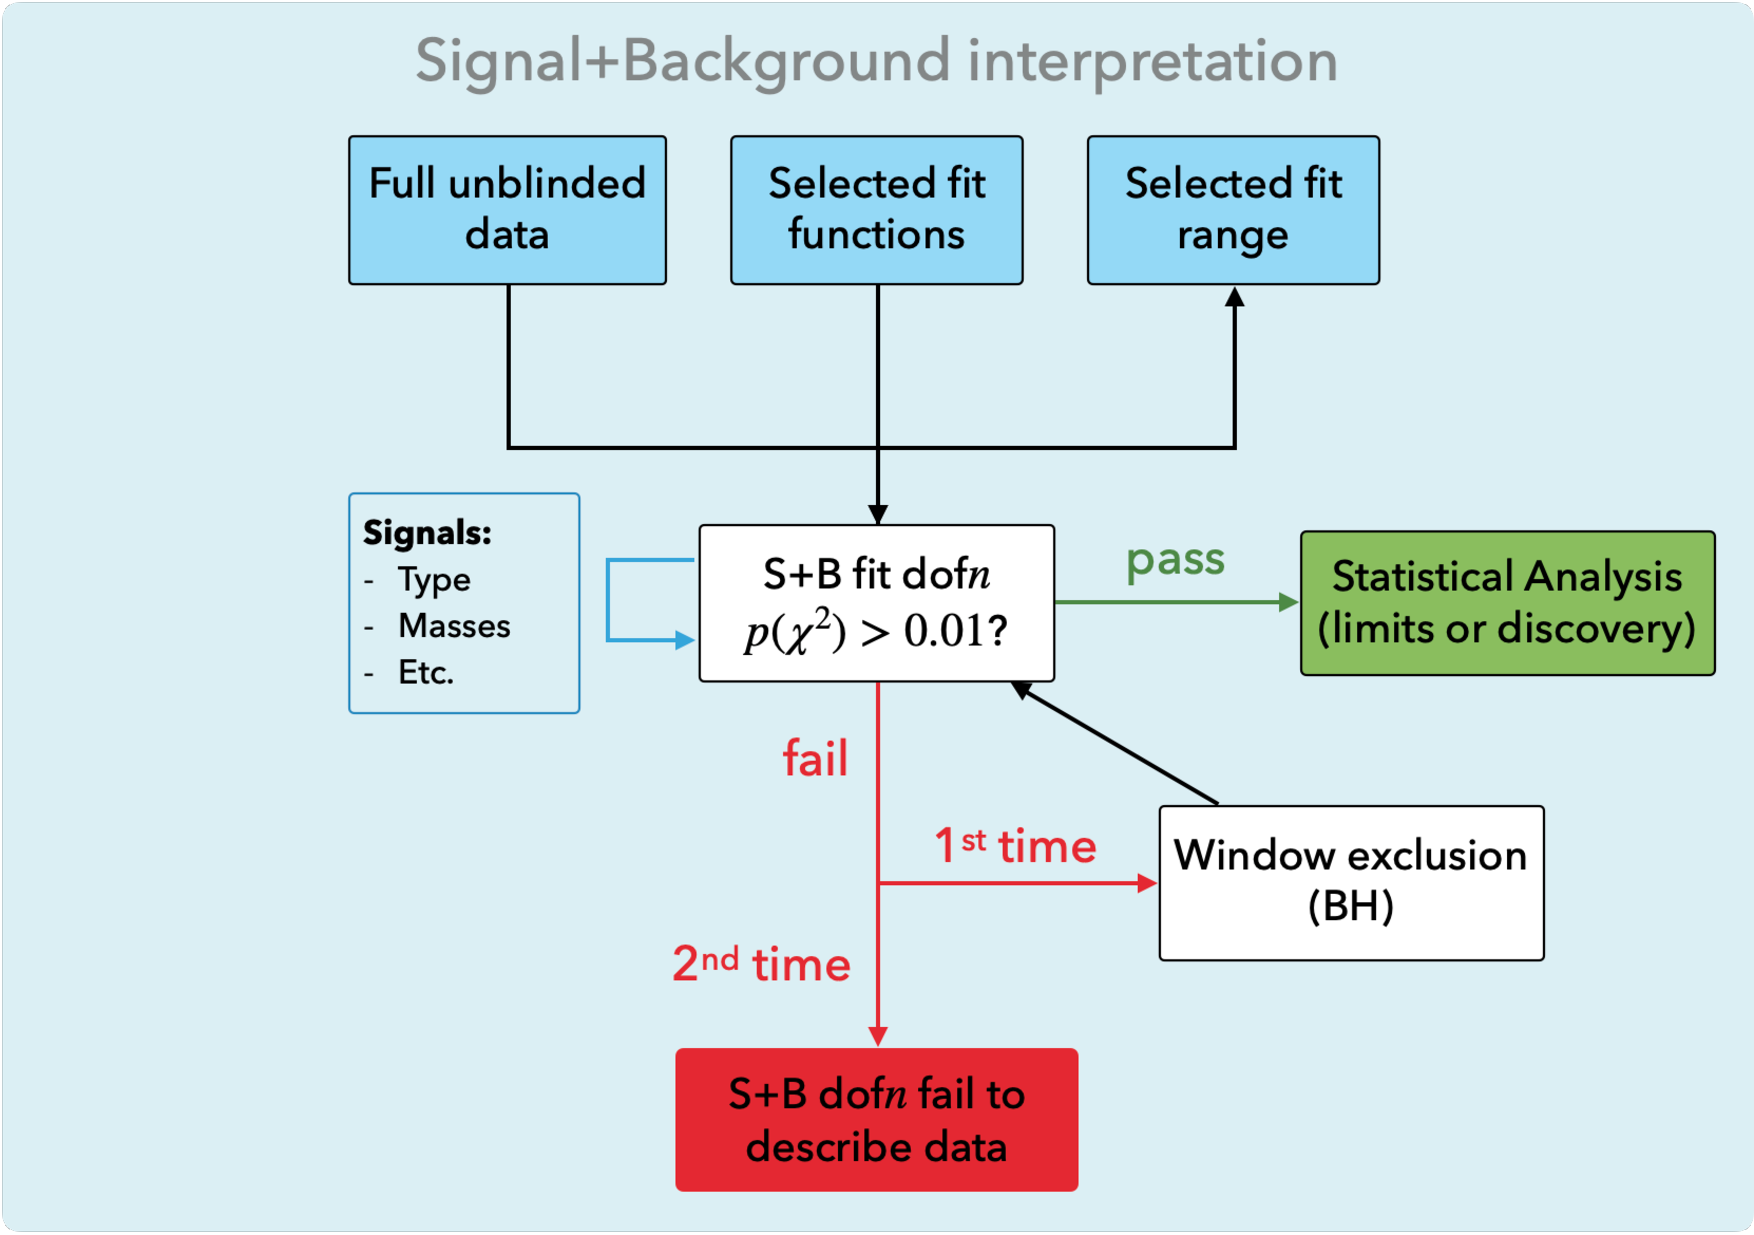
\includegraphics[width=0.7\linewidth]{5_resonances/results/sigbkg/unblind_strategy3_sb}
    \caption{Esquema del proceso utilizado para los ajustes \ac{SB} a los datos.}
    \label{fig:results:results:bkgsig:strat}
\end{figure}

El flujo para la interpretación de los resultados teniendo en cuenta las señales se esquematiza en la \Fig{\ref{fig:results:results:bkgsig:strat}}. Este proceso se repite para cada tipo de señal estudiada: \acf{EQ}, \acf{QBH} y resonancias gaussianas genéricas.
En primer lugar, se realiza un ajuste de \ac{SB} en la región de señal elegida seguido de un test de \chisq. Si el valor \(p\) del mismo supera el umbral de 0.01, indica un buen ajuste en todo el espectro y se inicia el procedimiento de establecimiento de límites. Si no se supera el umbral, puede deberse a un efecto local distinto de la hipótesis de la señal. En ese caso, se aplica una exclusión de ventana utilizando el algoritmo \bh como se ha descripto anteriormente y se repite el test de \chisq. Este camino es necesario para poder establecer límites en todo el rango \myj incluso si un único efecto localizado impidiera buenos ajustes para todas las demás hipótesis de señal a masas diferentes. Si en esta segunda prueba \(p(\chisq)\) supera el umbral de 0.01, el análisis estadístico continúa como en la otra ruta, sólo que con una ventana enmascarada. Si no se supera el umbral, el ajuste de \ac{SB} no describe correctamente a los datos y no se puede presentar ninguna interpretación.

El objetivo es establecer límites en los parámetros de la teoría, es decir, determinar la cantidad máxima de señal potencial para la que la hipótesis de \ac{SB} \(H_1\) proporciona una buena descripción de los datos en comparación con la hipótesis de \ac{BO} \(H_0\). Los límites se calculan a \(95\%\) \ac{CL} siguiendo el procedimiento descripto en la \Sect{\ref{subsec:strategy:stat_treatment:hypo_test}}.


\subsubsection{Límites a los diferentes modelos considerados}
\label{subsubsec:results:results:bkgsig:results}

En los párrafos siguientes, se ofrece una descripción de los resultados obtenidos para cada modelo de señal considerado en la presente tesis.

Los resultados de los límites superiores en términos de la sección eficaz visible de la señal están dados por
\begin{equation}
    \label{eq:results:results:bkgsig:results:visible_xs}
    \sigma_s \times \text{Br} \times A \times \varepsilon
\end{equation}
% en lugar de en la intesidad de la misma, \(\mu\) (la relación entre ambos se puede observar en la \Eqn{\ref{eq:strategy:stat_treatment:stat_model:mu_si}}).
% Esta forma de presentar los resultados es más común en casos donde las formas de las señales son genéricas y no se cuenta con medidas exactas de las aceptancias y/o eficiencias.
Dado que para las señales Gaussianas estudiadas en esta tesis uno no cuenta con eficiencias o aceptancias, los límites superiores para estas señales serán presentados en términos de la \Eqn{\ref{eq:results:results:bkgsig:results:visible_xs}}. Por otro lado, para los modelos teóricos con los que se cuenta con una simulación completa del mismo, se presentan los límites superiores en términos del producto entre la sección eficaz correspondiente y el \textit{branching ratio} \(\sigma_s \times \text{Br}\), como lo es en el caso de los modelos de \acp{EQ} y \acp{QBH}.


\paragraph{Quark excitados}
\label{paragraph:results:results:bkgsig:results:qstar}

El modelo \ac{EQ} propone un escenario en el que los quarks no son partículas fundamentales sino estados ligados que decaen rápidamente en un fotón y un quark del mismo sabor. Los resultados obtenidos en esta tesis son los primeros en el \ac{LHC}, que conducen a límites de los modelos de \ac{EQ} separados en tres sabores diferentes: \qstar, \cstar y \bstar.
Además, el acoplamiento de los \acp{EQ} con los campos de gauge del \ac{SM}, \(f=f'=f_s\), se mantiene como parámetro libre por lo que los límites se calculan en el plano acoplamiento-masa, dando lugar a límites bidimensionales.


\begin{figure}[ht!]
    \centering
    \begin{subfigure}[t]{0.49\linewidth}
        \centering
        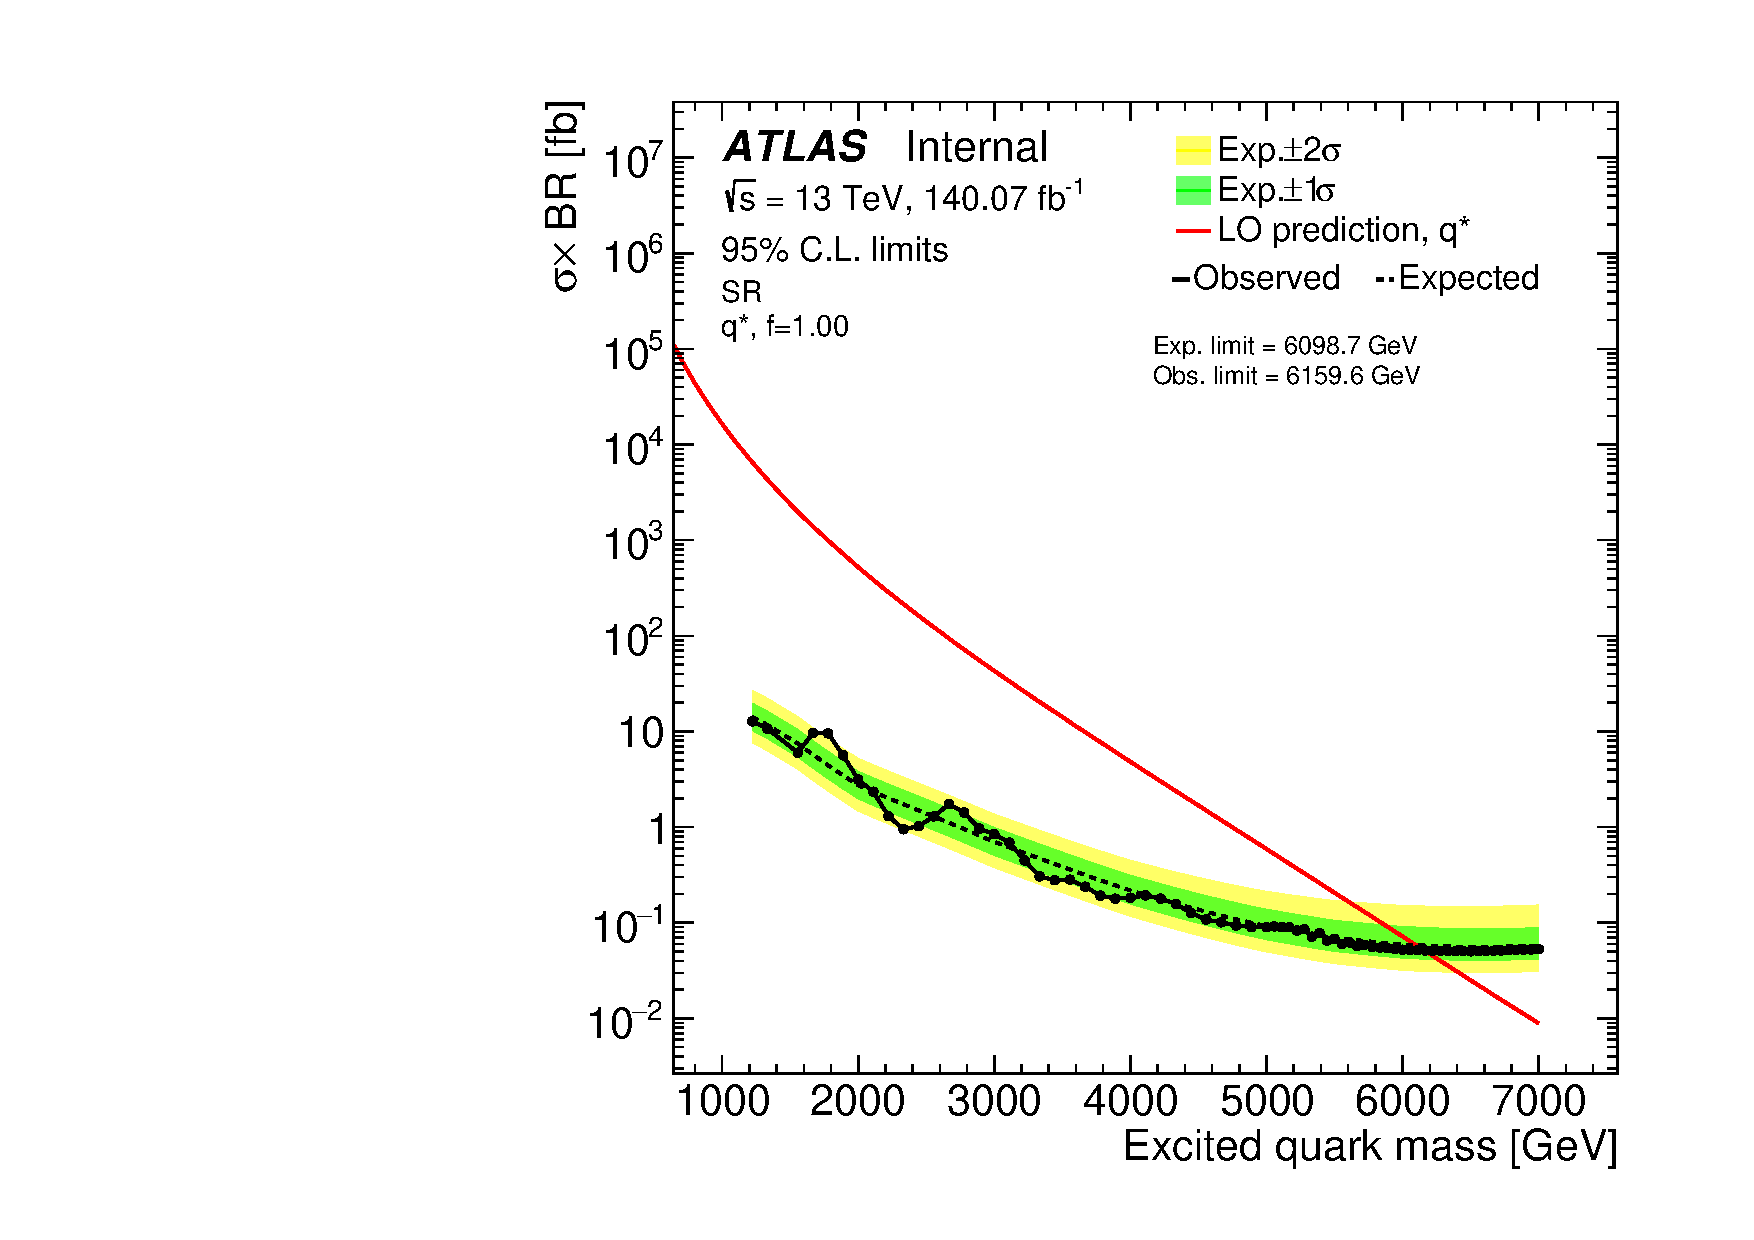
\includegraphics[width=\linewidth]{5_resonances/results/sigbkg/qstar/can__qstar__f1p00__q__SR__qstar__Run2}
        \caption{SR.}
        \label{fig:results:results:bkgsig:results:qstar:limits:SR}
    \end{subfigure}
    \hfill
    \begin{subfigure}[t]{0.49\linewidth}
        \centering
        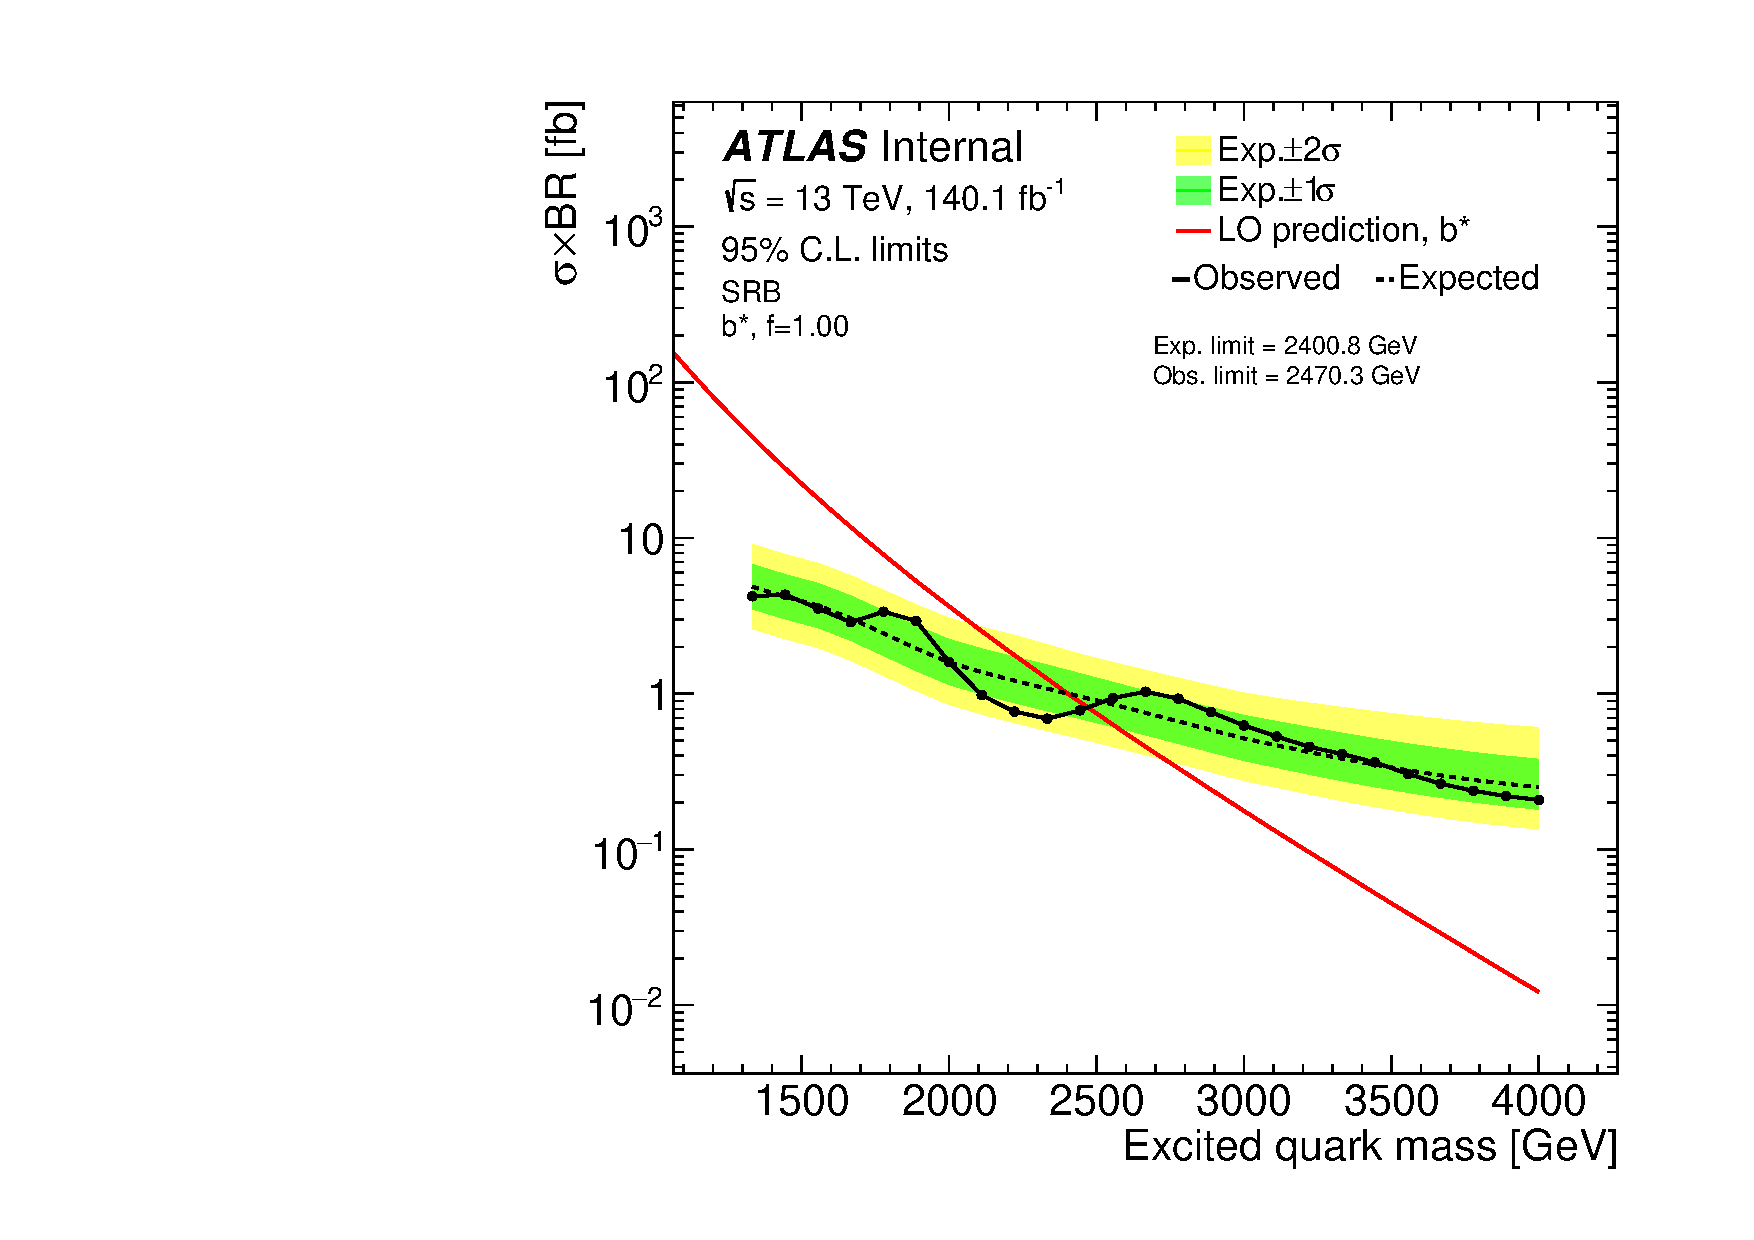
\includegraphics[width=\linewidth]{5_resonances/results/sigbkg/qstar/can__qstar__f1p00__b__SRB__qstar__Run2}
        \caption{SRB.}
        \label{fig:results:results:bkgsig:results:qstar:limits:SRB}
    \end{subfigure}\\
    \begin{subfigure}[t]{0.49\linewidth}
        \centering
        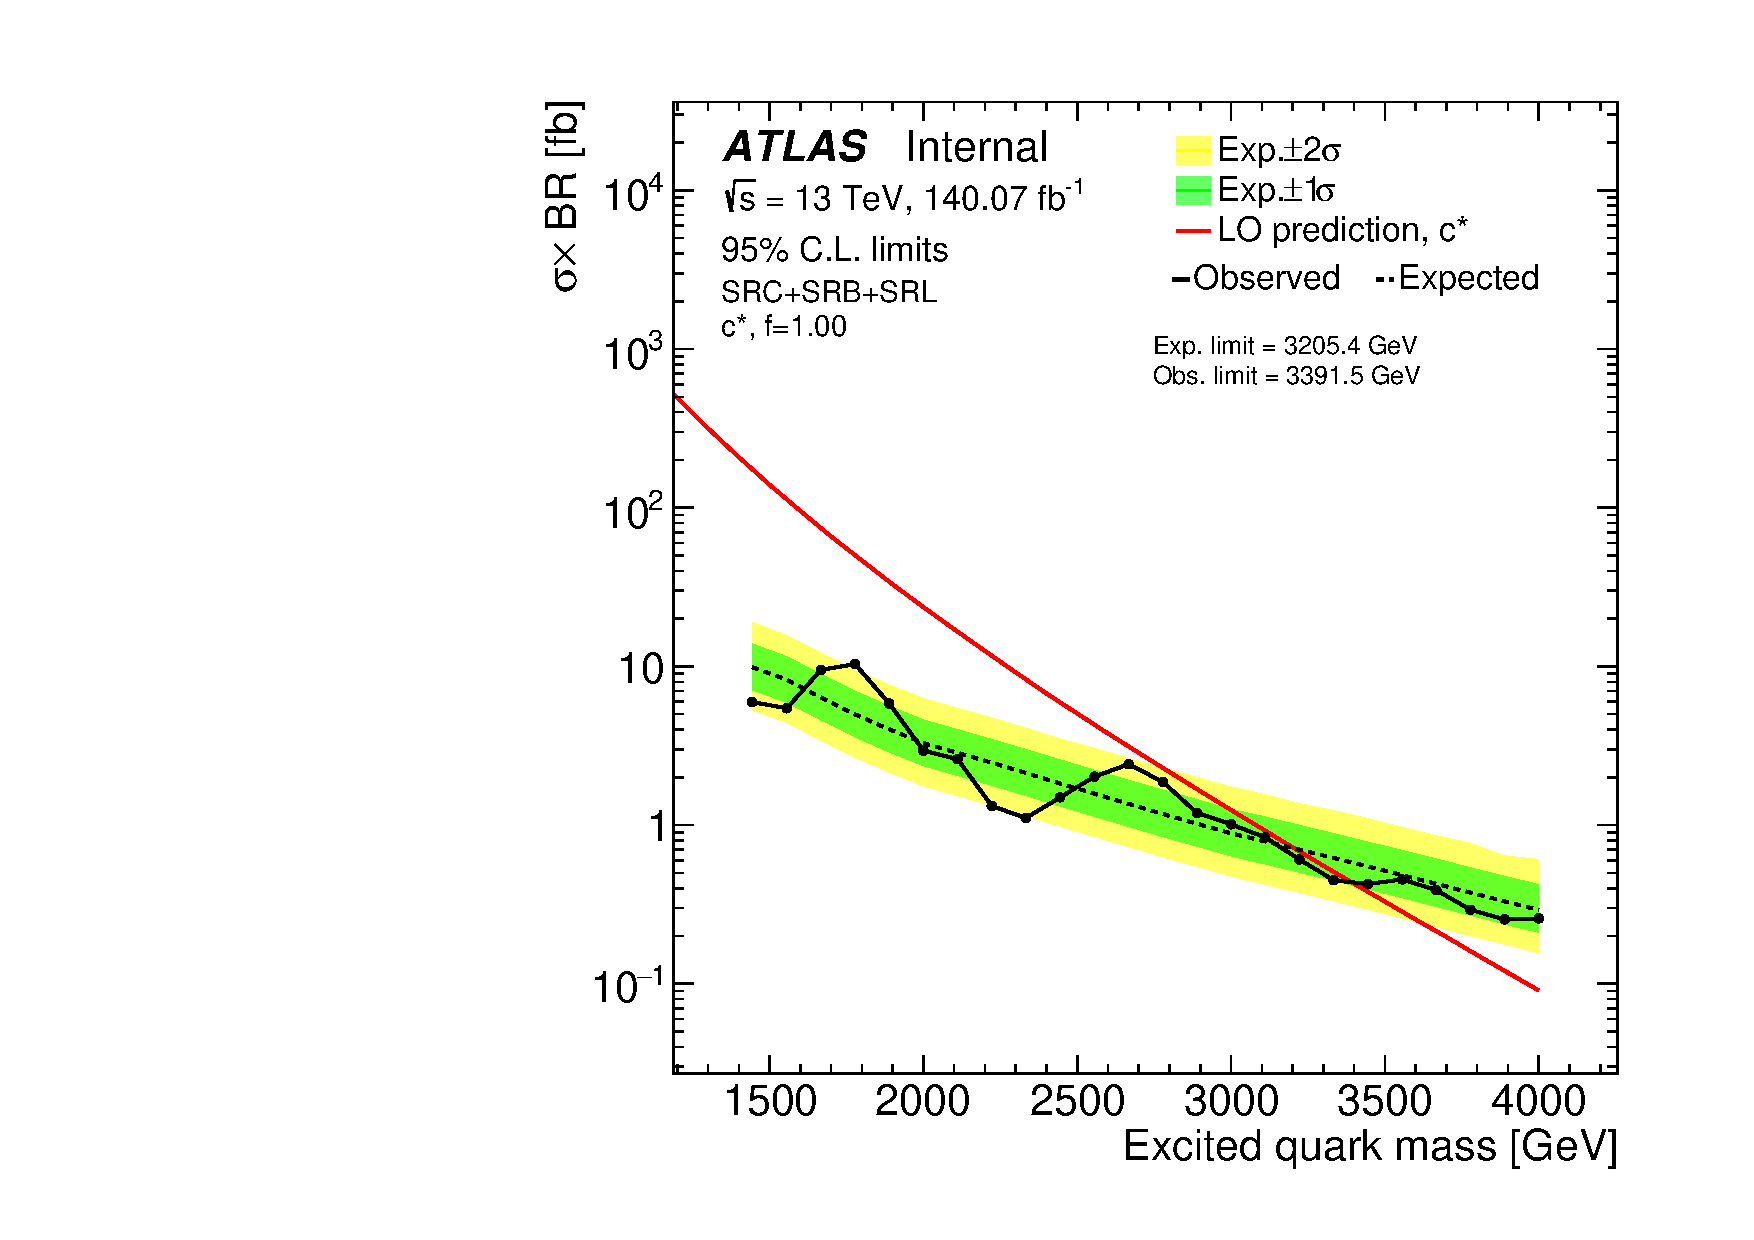
\includegraphics[width=\linewidth]{5_resonances/results/sigbkg/qstar/can__qstar__f1p00__c__SRC50_SRB_SRL50__qstar__Run2}
        \caption{SRC+SRB+SRL.}
        \label{fig:results:results:bkgsig:results:qstar:limits:SRC}
    \end{subfigure}
    \caption{Límites superiores observados y esperados en los modelos de señal de \qstar, \cstar and \bstar con acoplamiento \(f=1\), utilizando el conjunto completo de datos del Run-2. Los límites esperados son mostrados con las líneas punteadas negras, mientras que la línea sólida con los puntos negros representan los límites observados. Las incertezas correspondientes a \(1\sigma\) y \(2\sigma\) se muestran con las zonas sombreadas de color verde y amarillo, respectivamente. Las líneas rojas sólidas indican las secciones eficaces predichas por las teorías consideradas. En cada figura, se marcan los límites superiores en la masa del \ac{EQ}.}
    \label{fig:results:results:bkgsig:results:qstar:limits}
\end{figure}

Comenzando con el caso de las señales de \qstar, los límites superiores se obtienen en la región inclusiva SR y se calculan para diferentes valores de acoplamiento. Los resultados de los límites superiores esperados y observados en \(\sigma_s \times \text{Br}\) se muestran en la \Fig{\ref{fig:results:results:bkgsig:results:qstar:limits:SR}} para el caso de acoplamiento \(f=1.0\). Pueden observarse excesos locales en masas más bajas (\(\sim 1800~\gev\) y \(\sim 2600~\gev\)) pero siempre contenidos dentro de la incerteza del límite esperado de \(2\sigma\). Estos excesos también coinciden exactamente con los mismos lugares en los que se localizaron los bumps más significativos por el \bh en la \Fig{\ref{fig:results:results:bkgonly:fits:SR}}.

Para las señales de \bstar se utiliza la región SRB. Los límites superiores se muestran en la \Fig{\ref{fig:results:results:bkgsig:results:qstar:limits:SRB}}, donde nuevamente los límites observados se comportan de la misma manera que para la región SR: las mayores desviaciones de los límites esperados se dan en las masas donde se encontraron los bumps más significativos usando \bh.

Finalmente, por primera vez en el \ac{LHC}, se obtienen en este trabajo límites sobre las señales de \cstar en el estado final de \gammajet. Los límites superiores de las señales de \cstar se calculan en tres regiones ortogonales simultáneamente: SRC, SRB y SRL, y se muestran para el acoplamiento \(f=1\) en la \Fig{\ref{fig:results:results:bkgsig:results:qstar:limits:SRC}}. Una interpretación similar de las desviaciones de los límites observados es más difícil en este caso ya que el ajuste simultáneo combina las contribuciones de las tres regiones. Sin embargo, es útil visualizar los límites que se obtendrían en caso de utilizar sólo la región SRC en comparación con las tres simultáneamente. Esta comparación se muestra en la \Fig{\ref{fig:results:results:bkgsig:results:qstar:limits_SRC_comparison}} donde se observa una clara mejora que conduce a un aumento de aproximadamente \(\sim 200~\gev\) en los límites superiores de la masa \mc.

\begin{figure}[ht!]
    \centering
    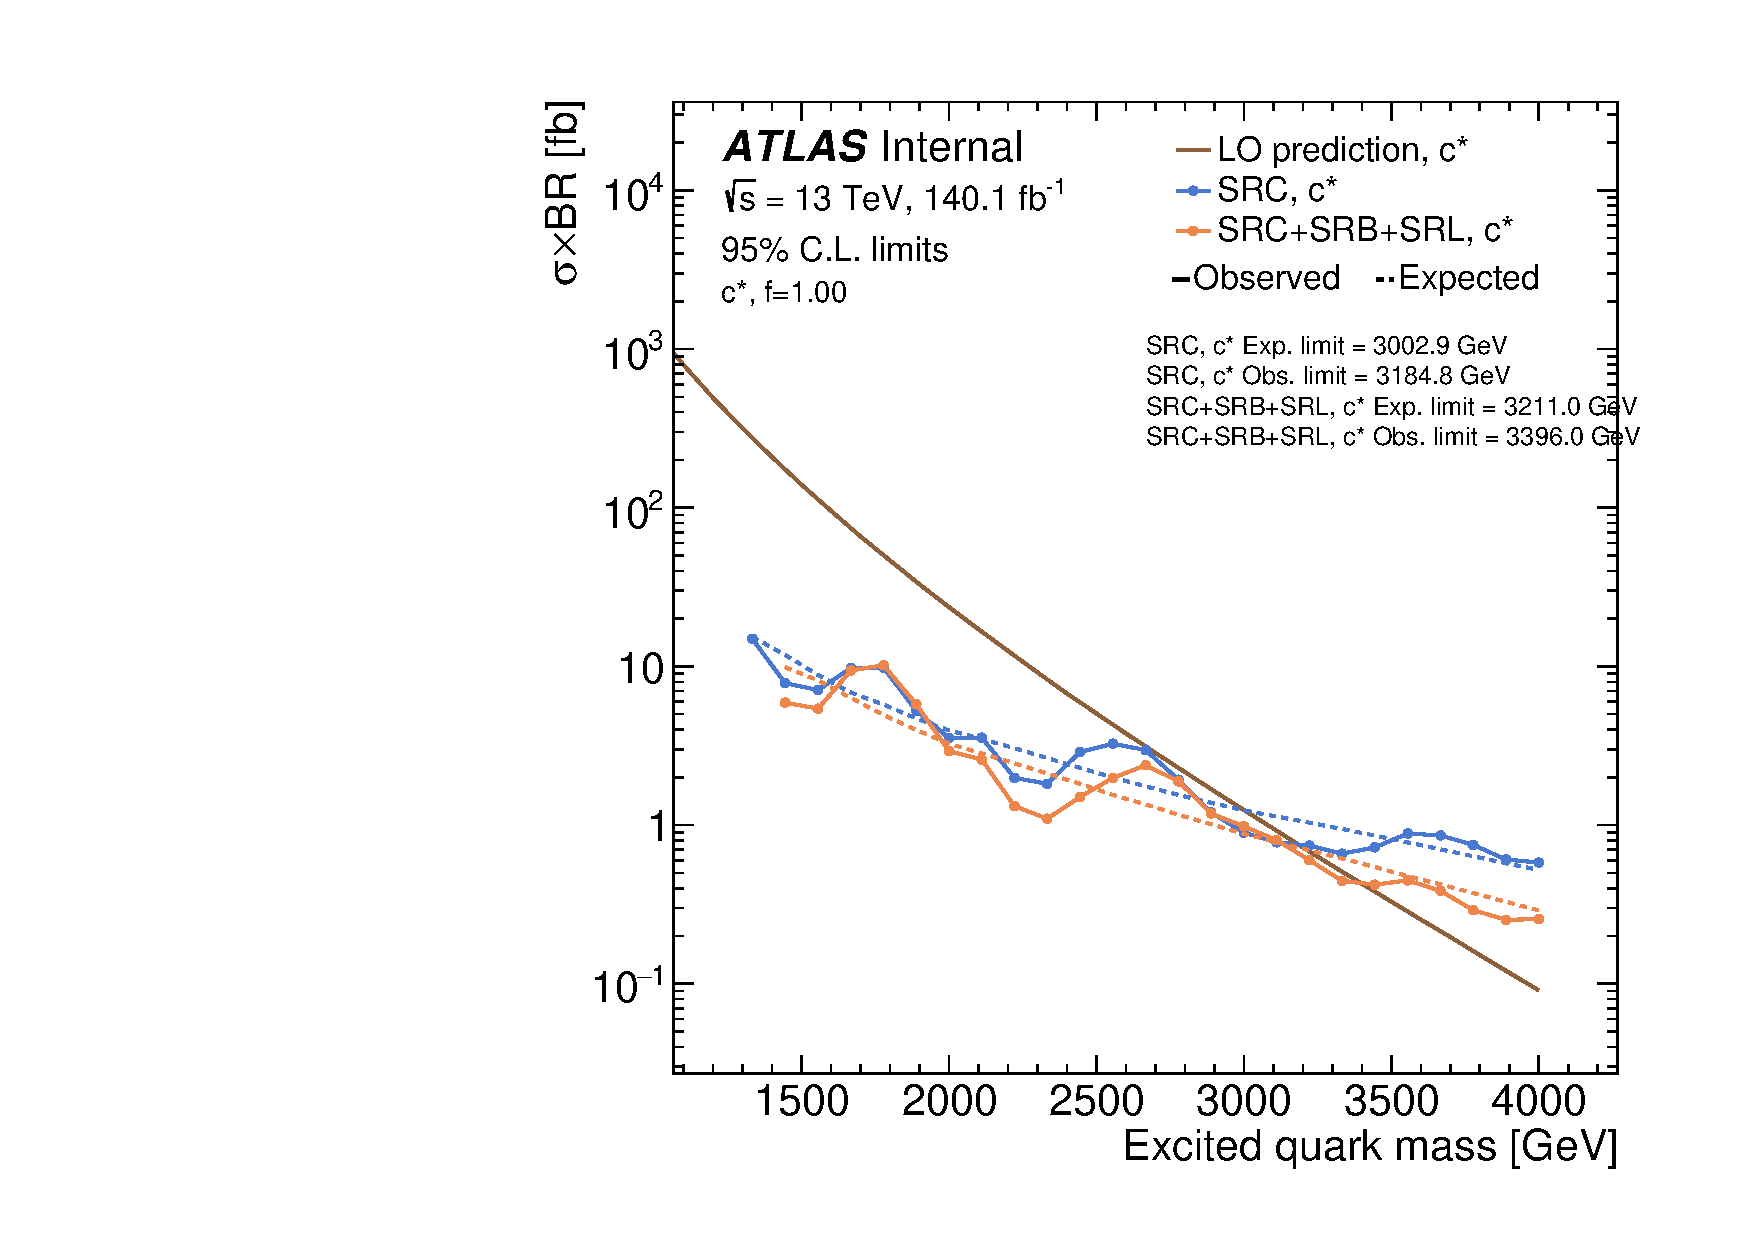
\includegraphics[width=0.49\linewidth]{5_resonances/results/sigbkg/qstar/can__qstar__f1p00__c____qstar__SRC50_SRC50_SRB_SRL50__Run2}
    \caption{Comparación de los límites superiores para las señales de \cstar calculado utilizando únicamente la región SRC (líneas azules) y utilizando las tres regiones SRC+SRB+SRL en simultáneo (líneas naranjas). Para los dos casos, se reportan los valores de los límites superiores en \mq.}
    \label{fig:results:results:bkgsig:results:qstar:limits_SRC_comparison}
\end{figure}

\begin{figure}[ht!]
    \centering
    \begin{subfigure}[t]{0.49\linewidth}
        \centering
        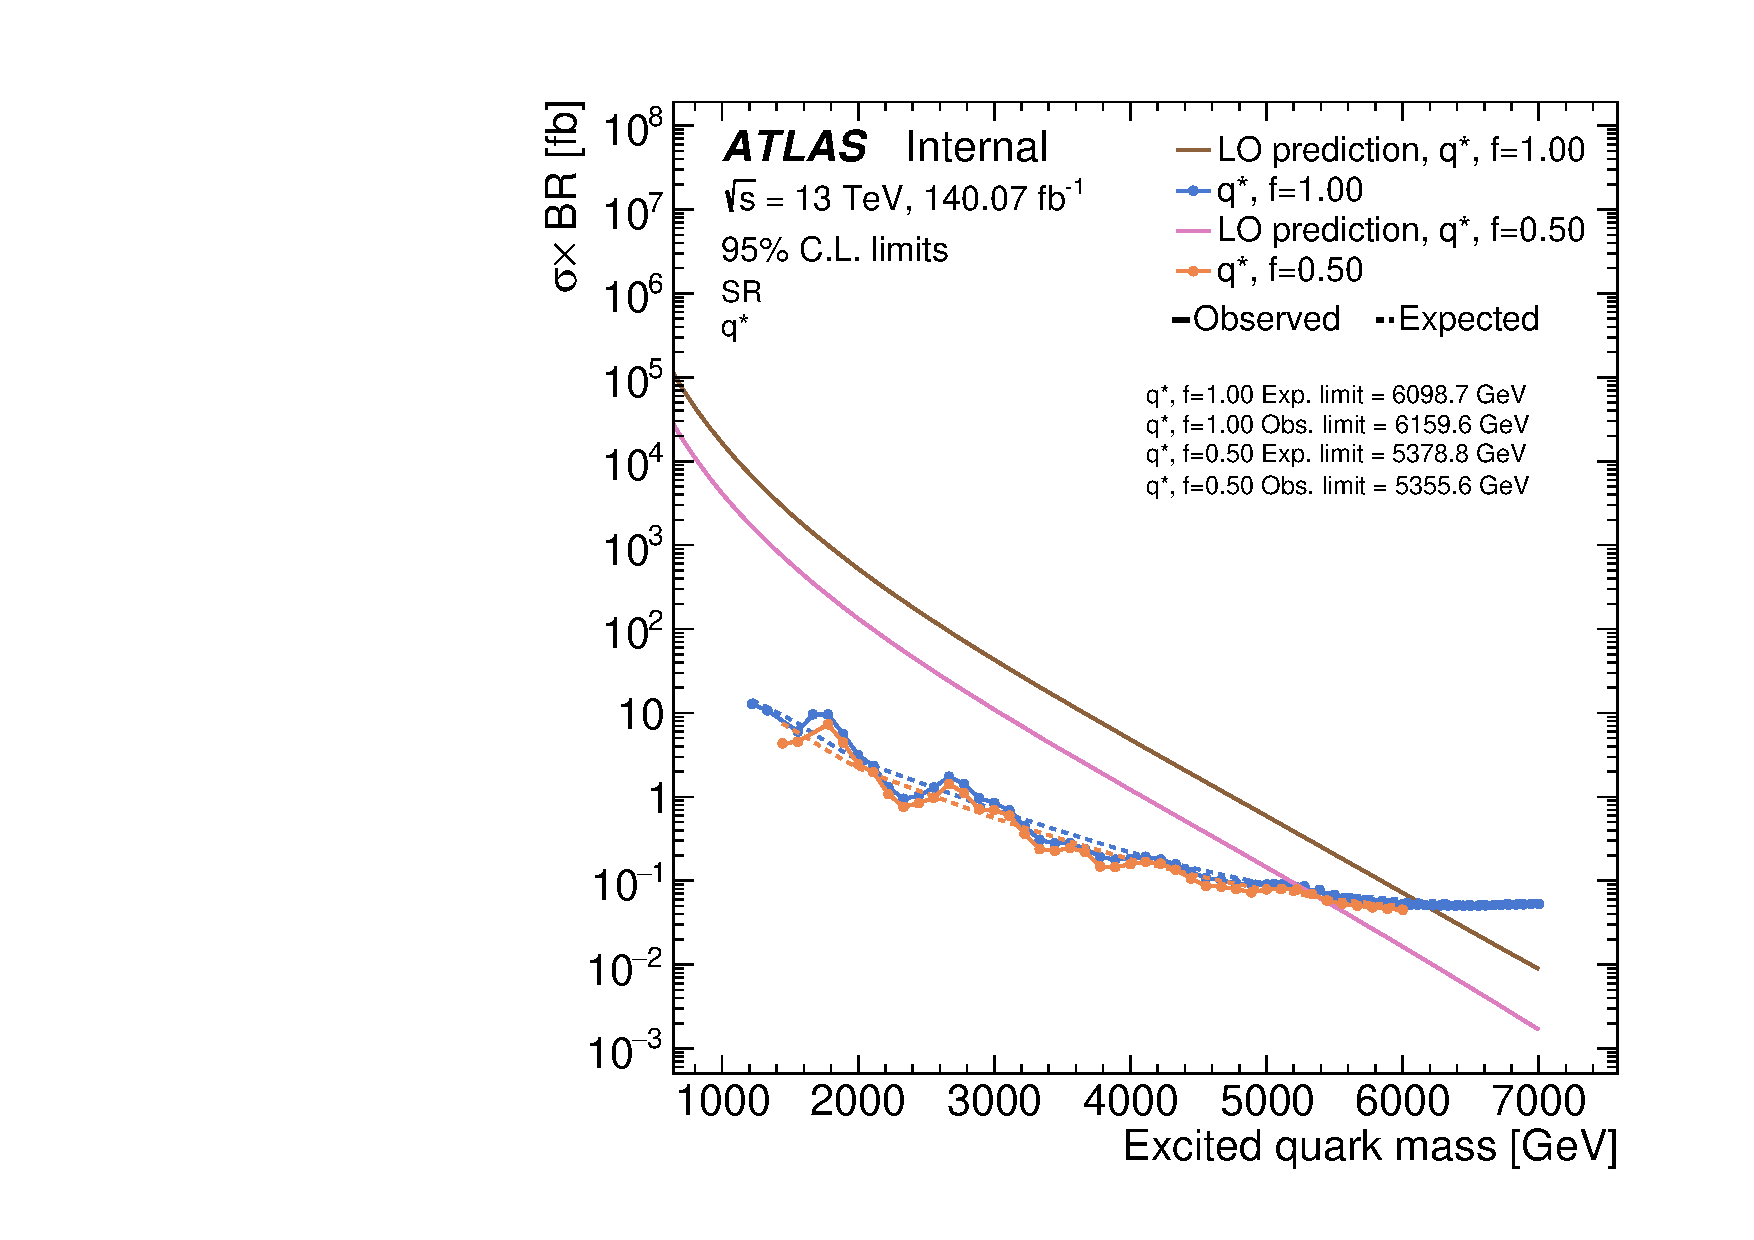
\includegraphics[width=\linewidth]{5_resonances/results/sigbkg/qstar/can__qstar__f1p00__q__SR__qstar__1p0_0p5__Run2}
        \caption{SR.}
        \label{fig:results:results:bkgsig:results:qstar:limits_couplings_comparison:SR}
    \end{subfigure}
    \hfill
    \begin{subfigure}[t]{0.49\linewidth}
        \centering
        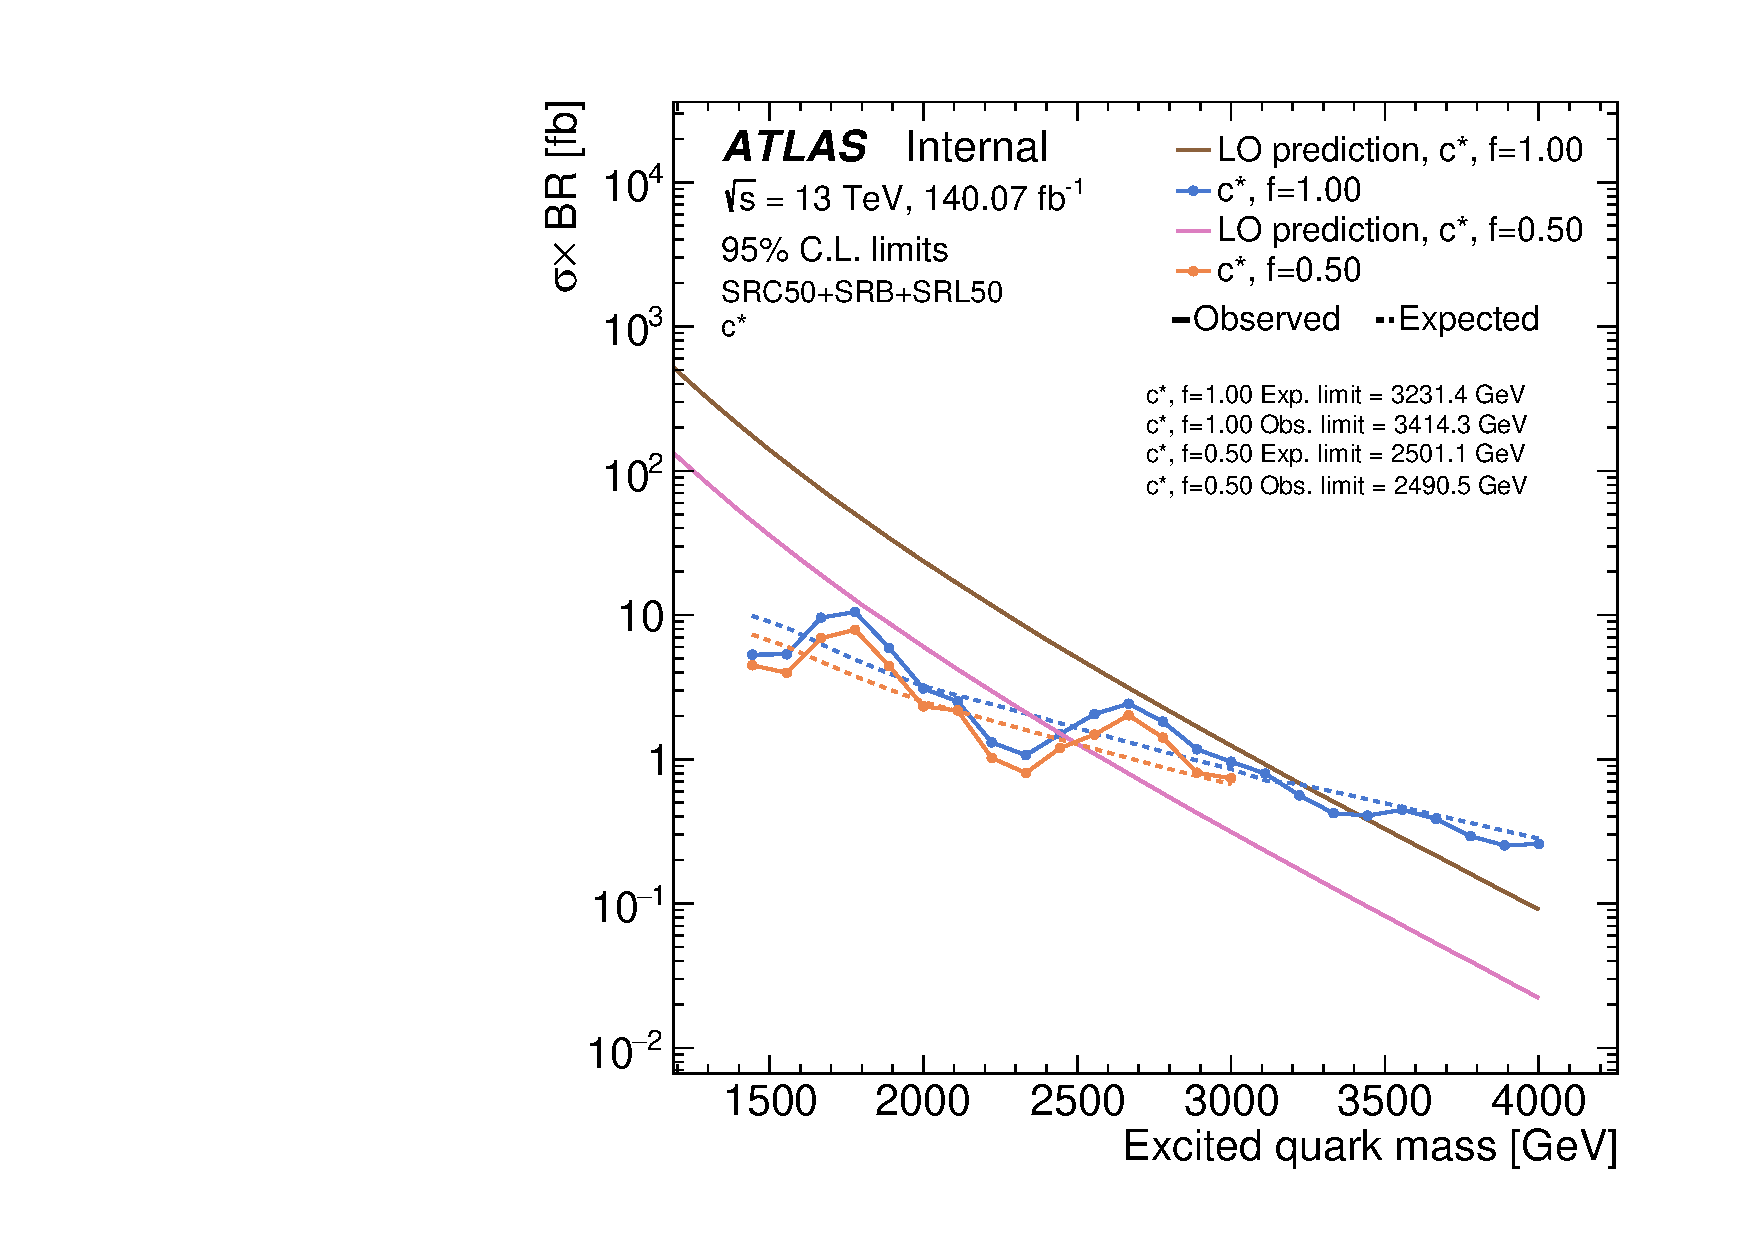
\includegraphics[width=\linewidth]{5_resonances/results/sigbkg/qstar/can__qstar__f1p00__c__SRC50_SRB_SRL50__qstar__1p0_0p5__Run2}
        \caption{SRC+SRB+SRL.}
        \label{fig:results:results:bkgsig:results:qstar:limits_couplings_comparison:SRC}
    \end{subfigure}\\
    \begin{subfigure}[t]{0.49\linewidth}
        \centering
        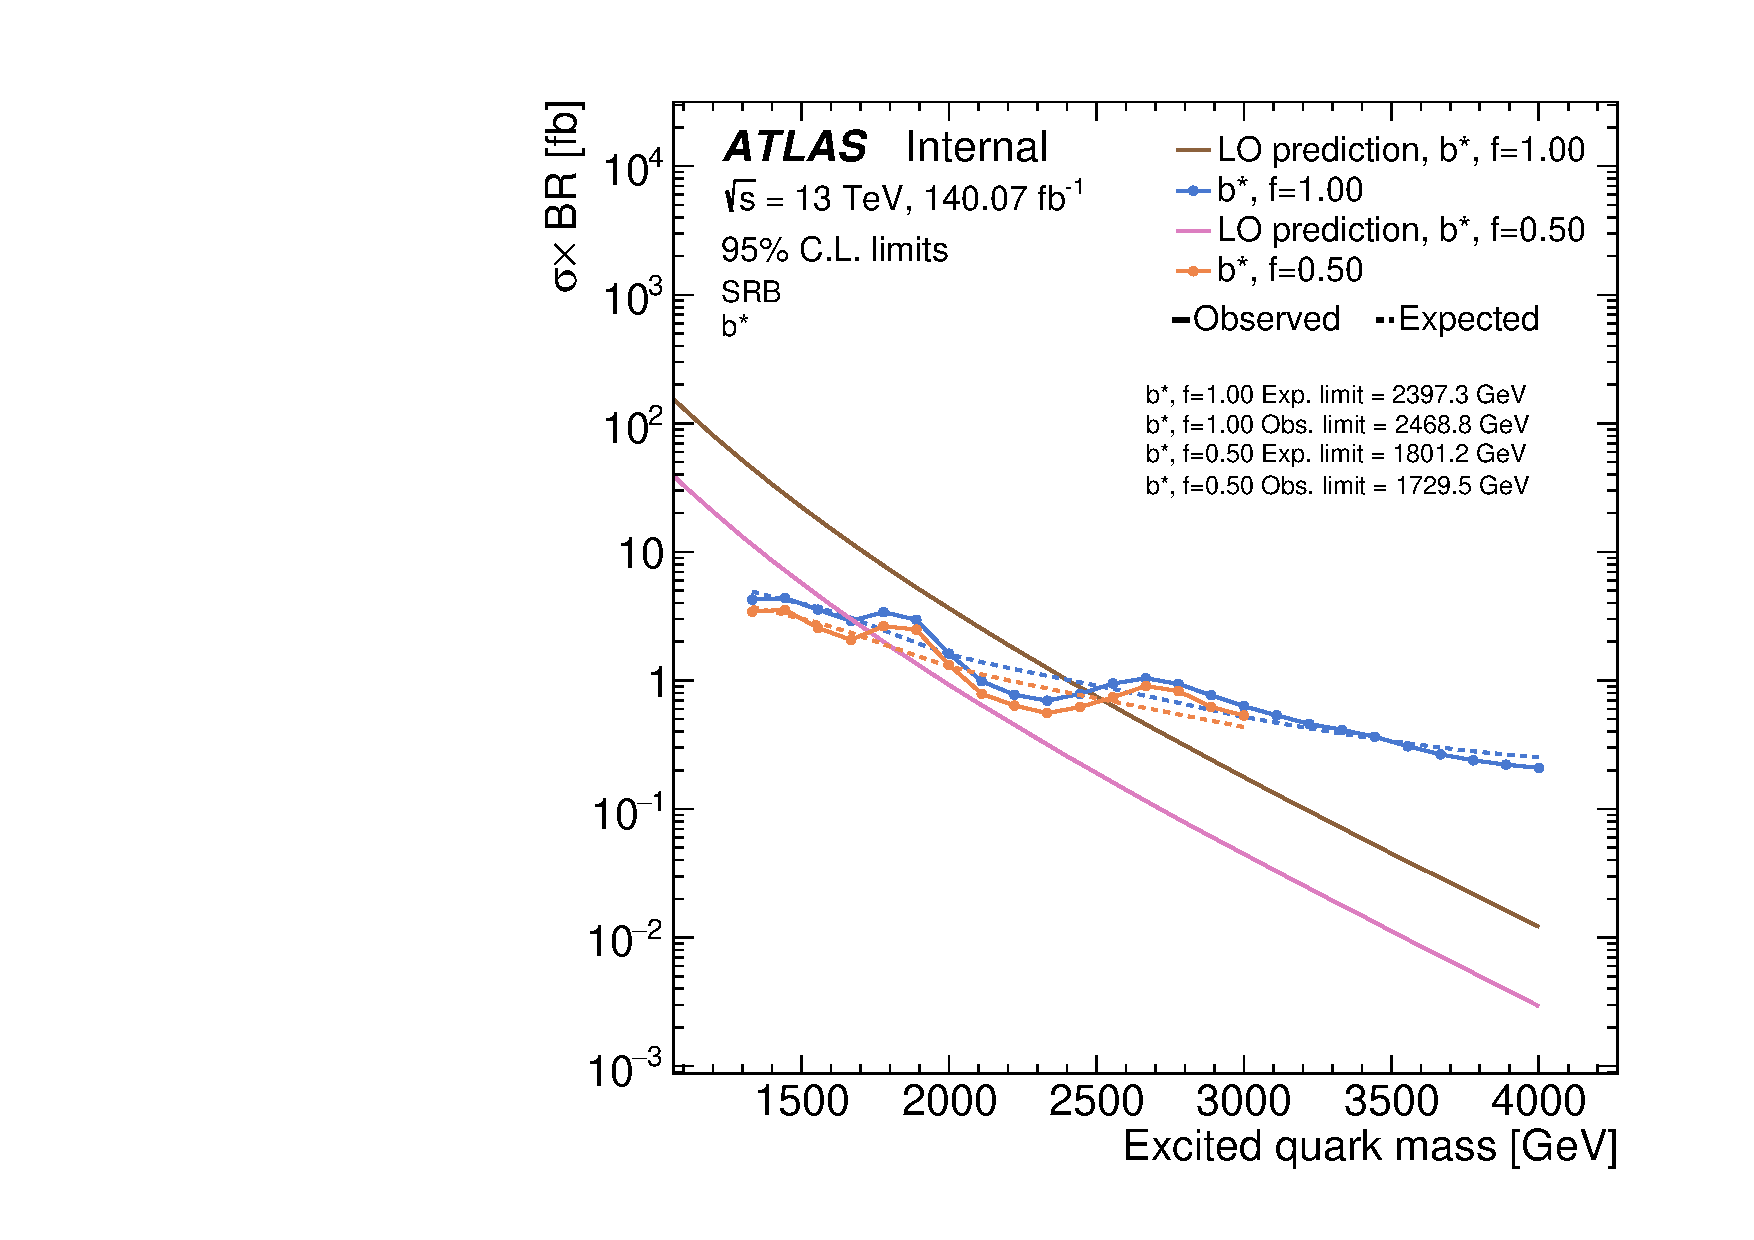
\includegraphics[width=\linewidth]{5_resonances/results/sigbkg/qstar/can__qstar__f1p00__b__SRB__qstar__1p0_0p5__Run2}
        \caption{SRB.}
        \label{fig:results:results:bkgsig:results:qstar:limits_couplings_comparison:SRB}
    \end{subfigure}
    \caption{Comparación de los límites observados y esperados entre señales con diferentes acoplamientos,para cada región del análisis. Las líneas azules (naranjas) representan los límites para acoplamientos de \(f=1\) (\(f=0.5\)), y los productos de sección eficaz y \textit{branching ratio} predichos por la teoría se muestran con la línea marrón (rosa).}
    \label{fig:results:results:bkgsig:results:qstar:limits_couplings_comparison}
\end{figure}

También es importante estudiar el comportamiento de los límites para distintos acoplamientos. En la \Fig{\ref{fig:results:results:bkgsig:results:qstar:limits_couplings_comparison}}, se muestran comparaciones de los límites superiores utilizando dos valores de acoplamiento diferentes. Para los tres sabores, la señal con menor acoplamiento siempre da los mejores límites en un factor pequeño y (casi) constante. Este comportamiento concuerda perfectamente con lo esperado dadas las diferentes aceptancias. Las formas de las señales de \acp{EQ} permanecen prácticamente inalteradas al variar el acoplamiento pero para \(f\ra 1\) aparece un pico secundario, producto de la producción \textit{off-shell} a más baja \myj, lo que conduce a aceptancias ligeramente menores.


Los límites superiores de \ac{EQ} pueden entonces representarse en el plano acoplamiento-masa, mostrando la exclusión en estos dos parámetros simultáneamente.
En el caso 2D, los límites superiores en el \(\sigma_s \times \text{Br}\) se representan mediante una superficie tridimensional y los límites superiores en los parámetros se obtienen de la intersección entre las predicciones y los límites superiores en \(\sigma_s \times \text{Br}\). Para encontrar la intersección se requiere que ambas superficies sean suaves y esto no es el caso para los valores de los límites superiores dado que se cuenta con un número finito señales. Utilizando las interpolaciones de las señales descriptas en \Sect{\ref{sec:signals:modeling}}, es posible lograr una superficie suave y casi continua de los límites logrando entonces poder realizar una interpolación de la intersección de ambas superficies. Estos límites superiores en los parámetros se muestran en la \Fig{\ref{fig:results:results:bkgsig:results:qstar:limits_2d}}. Aquí, se muestran los límites superiores observados y esperados a \(95\%\) \ac{CL} (con la banda de incerteza \(\pm 1 \sigma\)) para los tres sabores considerados, en sus respectivas regiones. Como era de esperar, los límites del modelo \qstar son aproximadamente dos veces más estrictos que los del modelo \cstar, que a su vez, son más estrictos que para la señal \bstar. Esta jerarquía en los límites es consecuencia principalmente de la sección eficaz de los procesos, ya que se esperan secciones eficaces más bajas para las resonancias más pesadas.

\begin{figure}[ht!]
    \centering
    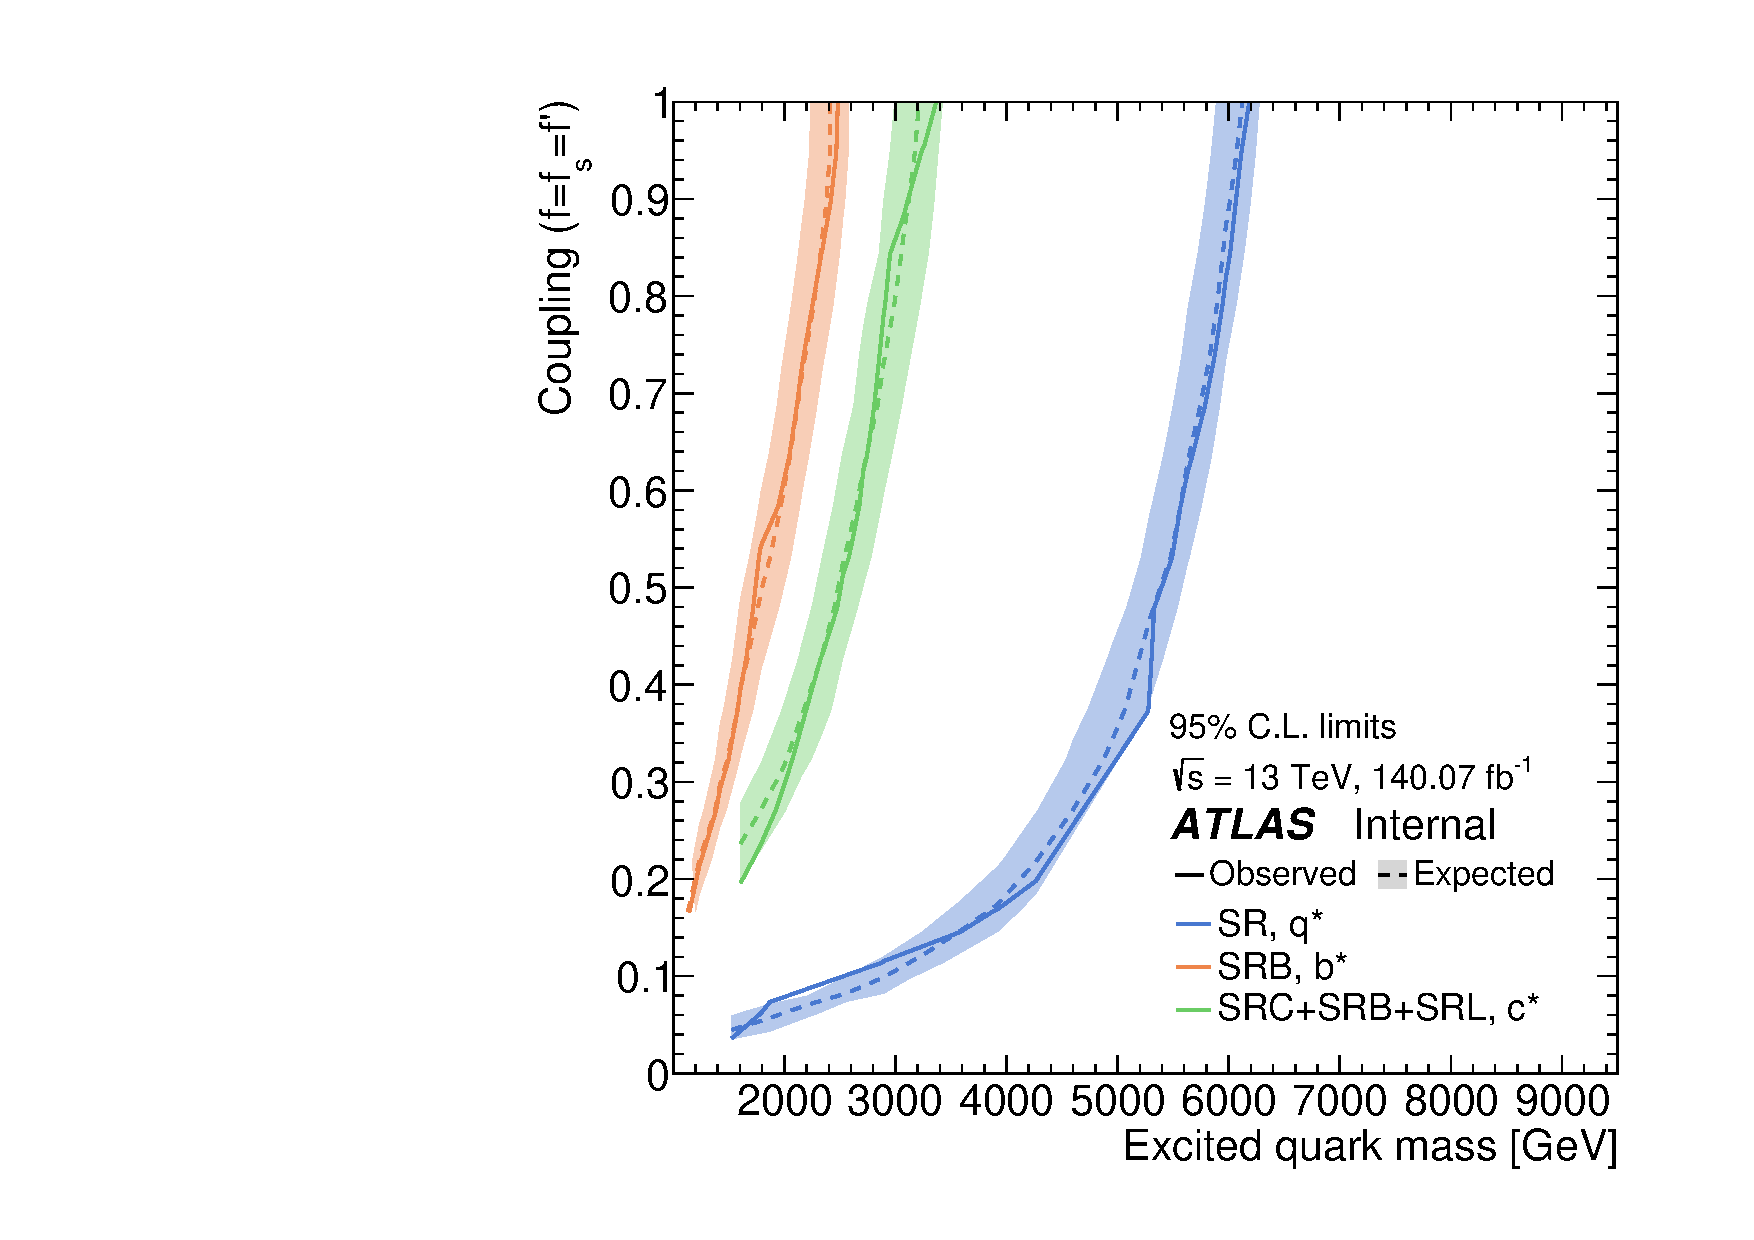
\includegraphics[width=0.9\linewidth]{5_resonances/results/sigbkg/qstar/can__qstar__q_b_c____qstar__SR_SRB_SRC50_SRB_SRL50__Run2}
    \caption{Límites esperados y observados en el plano de acoplamiento-masa para los modelos de \qstar (SR), \bstar (SRB) y \cstar (SRC+SRB+SRL). Los límites esperados (observados) se muestran con líneas punteadas (sólidas), y la región de incerteza de \(1\sigma\) se muestran como las zonas sombreadas.}
    \label{fig:results:results:bkgsig:results:qstar:limits_2d}
\end{figure}

Los límites superiores obtenidos en este análisis son los más estrictos hasta la fecha para el estado final \gammajet. En el caso de acoplamiento \(f=1\), los datos excluyen los modelos de \qstar, \cstar y \bstar con masas de hasta \(6159.6\), \(3391.5\) y \(2468.8~\gev\), respectivamente.



\paragraph{Micro Agujeros Negros}
\label{paragraph:results:results:bkgsig:results:qbh}

Al igual que para los límites de exclusión de \ac{EQ}, los límites superiores para los \ac{QBH} se indican en términos de la sección eficaz por el \textit{branching ratio} \(\sigma_s \times \text{Br}\).
Los resultados sobre los límites observados y esperados para los dos modelos de \ac{QBH}, RS1 y ADD se muestran en la \Fig{\ref{fig:results:results:bkgsig:results:qbh:limits}}. Siguiendo el resumen de estrategias para los ajustes presentado en la \Tab{\ref{tab:bkg:modeling:strategy_modeling:summary}}, las señales de \ac{QBH} sólo se interpretan en la región inclusiva SR. De forma similar a lo observado en el caso de las señales de \ac{EQ}, los límites observados en \(\sim 1800~\gev\) y \(\sim 2600~\gev\) presentan desviaciones de hasta \(2\sigma\) debido a los excesos locales (no significativos) encontrados en los datos con \bh.

\begin{figure}[ht!]
    \centering
    \begin{subfigure}[h]{0.49\linewidth}
        \centering
        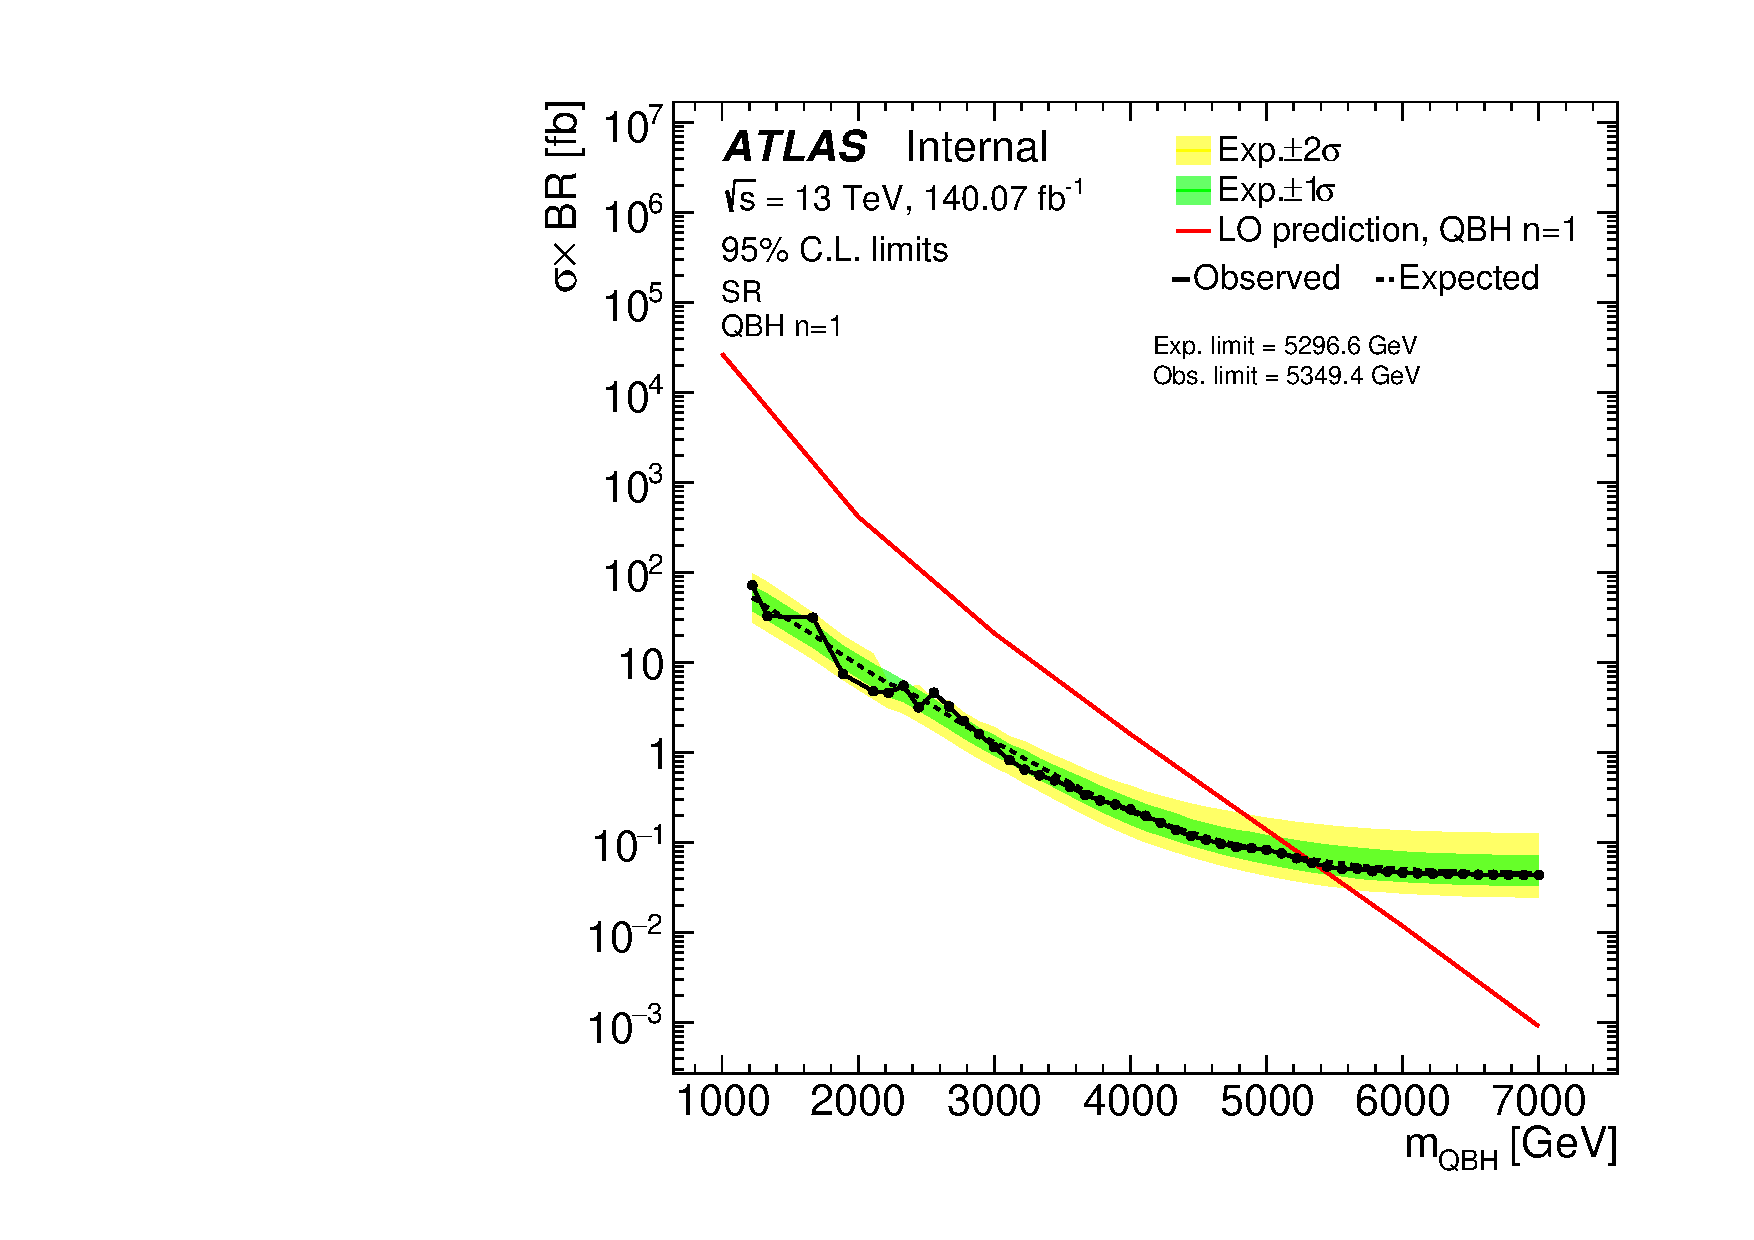
\includegraphics[width=\linewidth]{5_resonances/results/sigbkg/QBH/n1/can__QBH__n1__n1____QBH__SR__Run2}
        \caption{RS1 (\(n=1\)) \ac{QBH} model.}
    \end{subfigure}
    \hfill
    \begin{subfigure}[h]{0.49\linewidth}
        \centering
        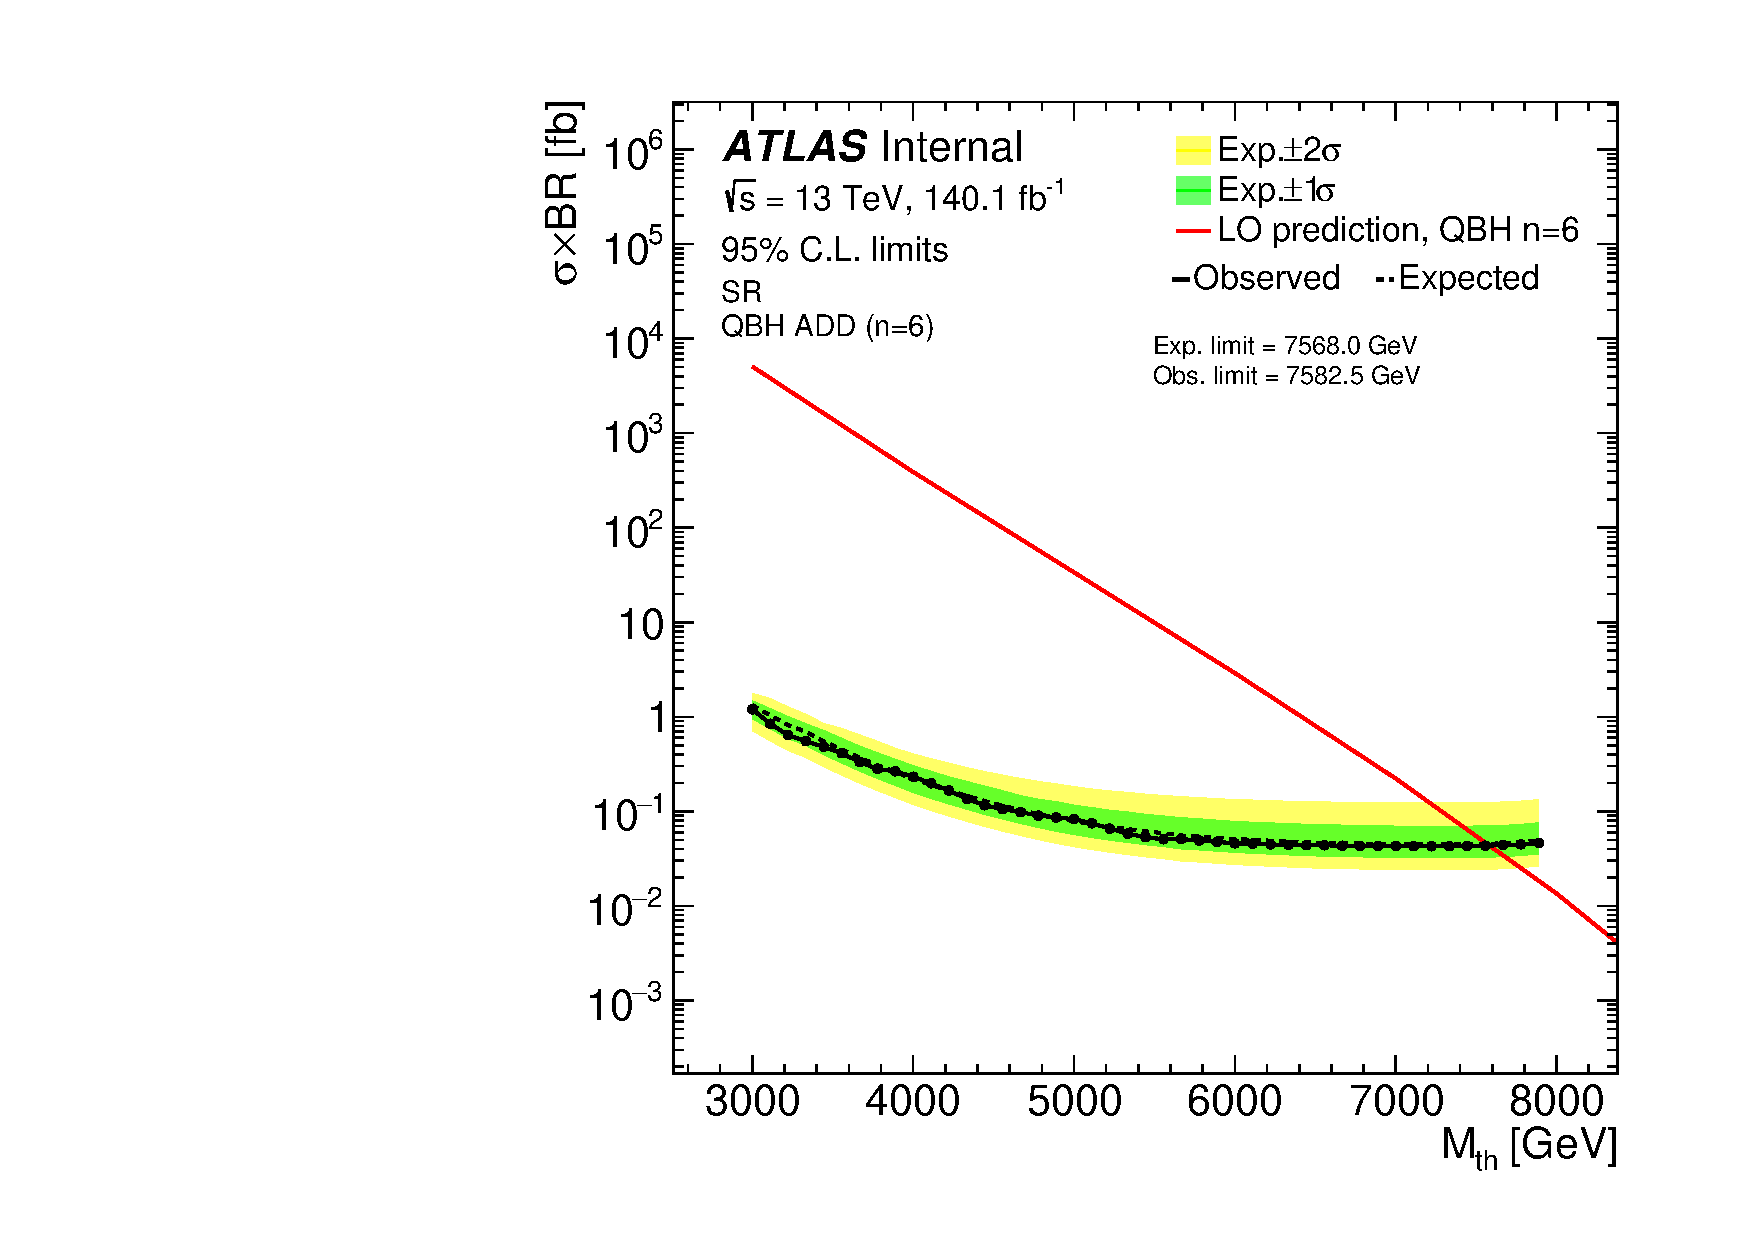
\includegraphics[width=\linewidth]{5_resonances/results/sigbkg/QBH/n6/can__QBH__n6__n6____QBH__SR__Run2}
        \caption{ADD (\(n=6\)) \ac{QBH} model.}
    \end{subfigure}
    \caption{Límites superiores observados y esperados para los modelos de \acp{QBH}. Los límites para el modelo RS1 (\(n=1\)) se muestra en la figura de la izquierda, mientras que para el modelo ADD (\(n=6\)) los resultados se presentan en la figura de la derecha. Los límites observados se muestran con los puntos y líneas negras sólidas. En cambio, los límites esperados están representados por las líneas punteadas negras, y las incertezas de \(\pm 1\) y \(\pm 2 \sigma\) se muestran con las zonas sombreadas de verde y amarillo, respectivamente.}
    \label{fig:results:results:bkgsig:results:qbh:limits}
\end{figure}

Los límites superiores de las masas de \acp{QBH} obtenidos son los más estrictos hasta la fecha en el estado final \gammajet. Los modelos que proponen dimensiones extra, ya sea con geometría deformada como en el modelo RS1, o con al menos dos dimensiones extra planas como en el modelo ADD, sugieren la formación de \ac{QBH}, y estas pueden excluirse con un \ac{CL} del \(95\%\) hasta masas de \(5349.4~\gev\) y \(7581.2~\gev\), respectivamente.




\paragraph{Modelos Gaussianos genéricos}
\label{paragraph:results:results:bkgsig:results:gaus}


El último modelo de señal considerado son las formas gaussianas genéricas. Estas señales permiten una interpretación general y agnóstica del modelo en este estado final. Los límites superiores esperados y observados se calculan con resonancias de forma gaussiana, en los cuales los anchos se eligen en un \(2\%\), \(7\%\) y \(15\%\) de la resolución de masa invariante. A diferencia de los modelos anteriores, los límites de exclusión reportados se refieren a la sección eficaz visible dada por la \Eqn{\ref{eq:results:results:bkgsig:results:visible_xs}} ya que pueden interpretarse para cualquier modelo arbitrario de señal que produzca una resonancia \gammajet de forma aproximadamente gaussiana en \myj.

Para cada una de las regiones de señal consideradas para este modelo de señal (SR, SRL, SRC y SRB), los resultados de los límites se muestran en la \Fig{\ref{fig:results:results:bkgsig:results:gaus:limits}}.
Los límites obtenidos en la región inclusiva SR muestran exactamente la misma estructura a bajo \myj que los otros modelos de señal, donde se observa un pequeño exceso de eventos de datos a \(\sim 1800~\gev\) y \(\sim 2500~\gev\).

La sensibilidad para resonancias más estrechas es mejor que para resonancias más anchas por dos razones: para resonancias anchas, el mismo número de eventos de señal se distribuye a través de un rango de \myj mayor lo que reduce la relación señal/fondo en este rango. Además, la flexibilidad del ajuste del fondo le permite adaptarse mejor a señales anchas que a señales estrechas provocando una mayor ambigüedad entre los eventos de señal y los de fondo.

A partir de la comparación de los distintos anchos, también es importante señalar que las resonancias estrechas producen muchas más fluctuaciones en los límites. Esto se debe a que los picos estrechos pueden captar más fácilmente cualquier fluctuación estadística en los datos y estas fluctuaciones se traducen en los límites. Por el contrario, las señales más anchas dan lugar a formas mucho más suaves en los límites observados.

\begin{figure}[ht!]
    \centering
    \begin{subfigure}[h]{0.49\linewidth}
        \centering
        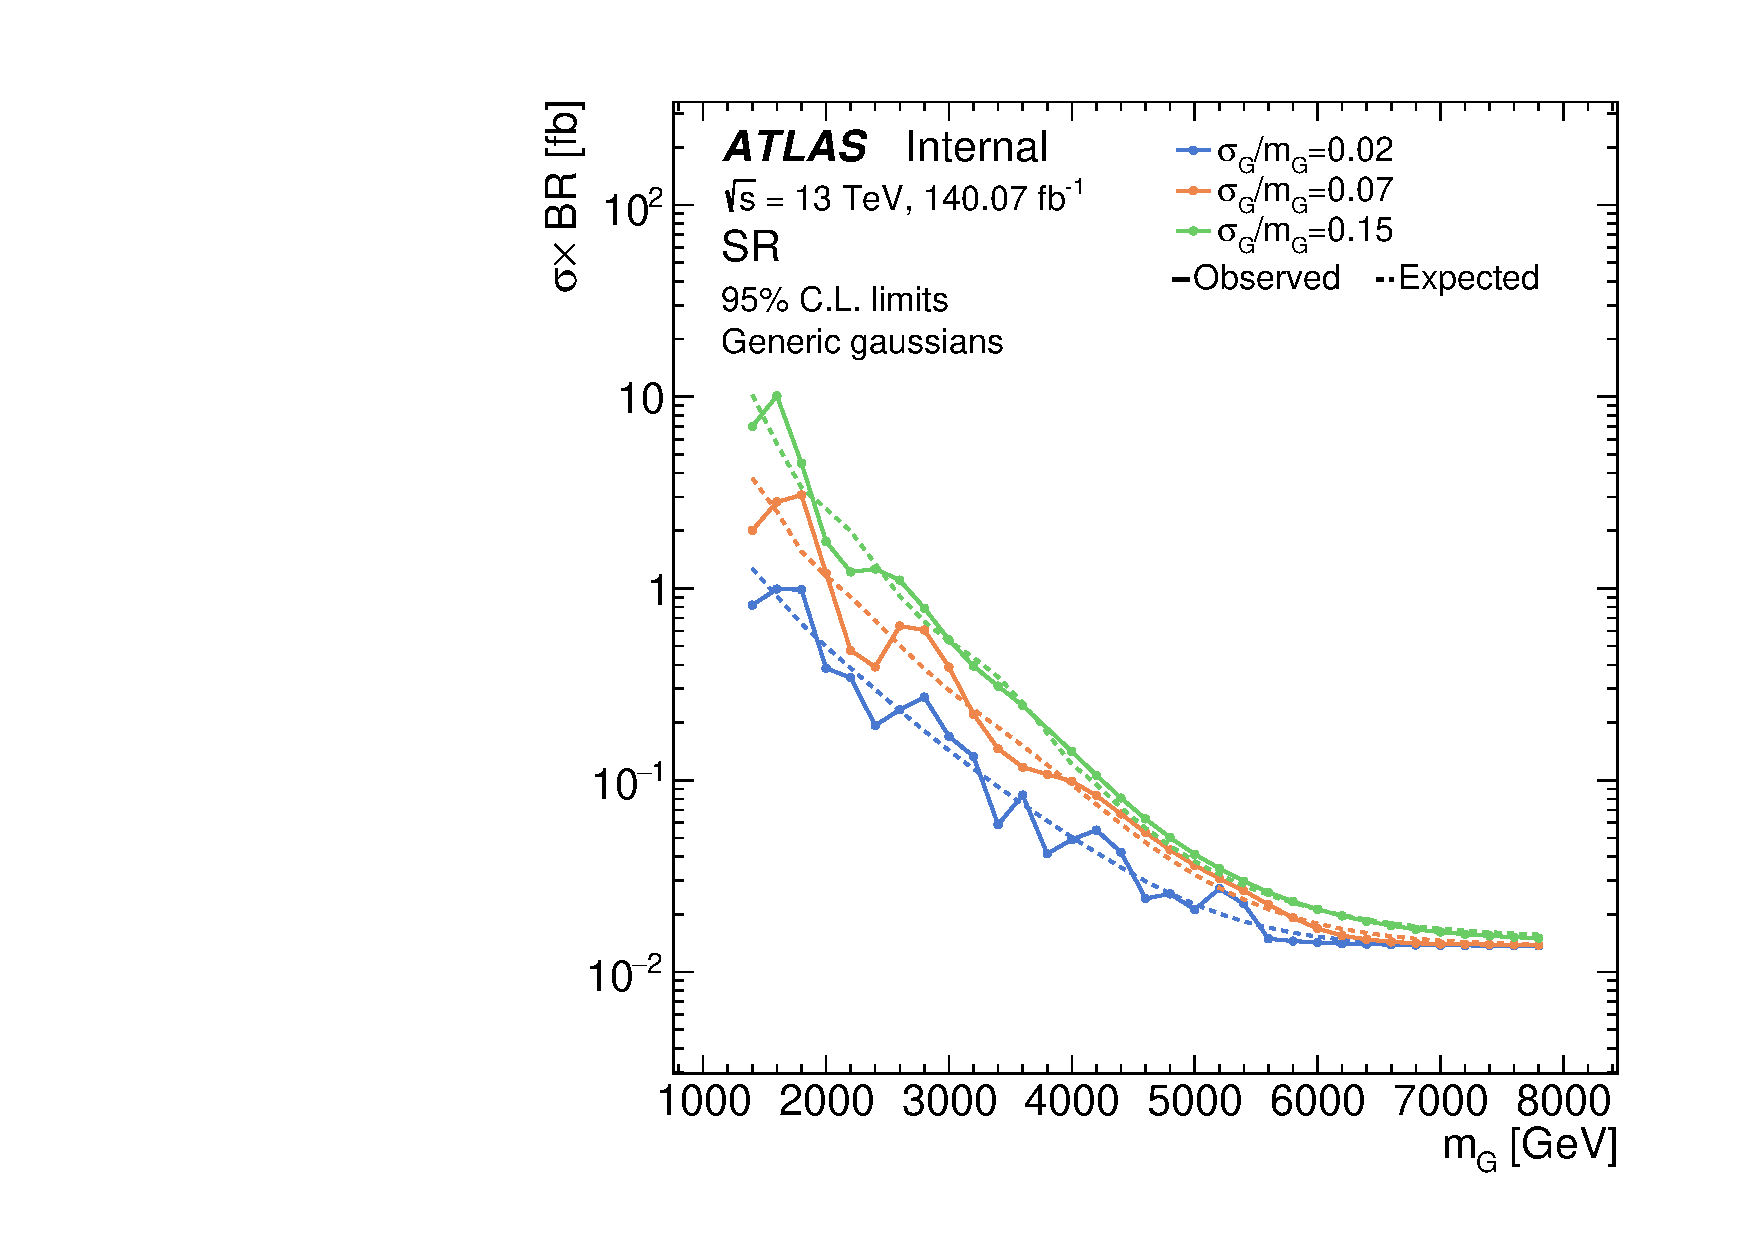
\includegraphics[width=\linewidth]{5_resonances/results/sigbkg/gaus/region/SR/can__gaus__SR____SR__gaus__width0p02_width0p07_width0p15__Run2}
        \caption{SR.}
    \end{subfigure}
    \begin{subfigure}[h]{0.49\linewidth}
        \centering
        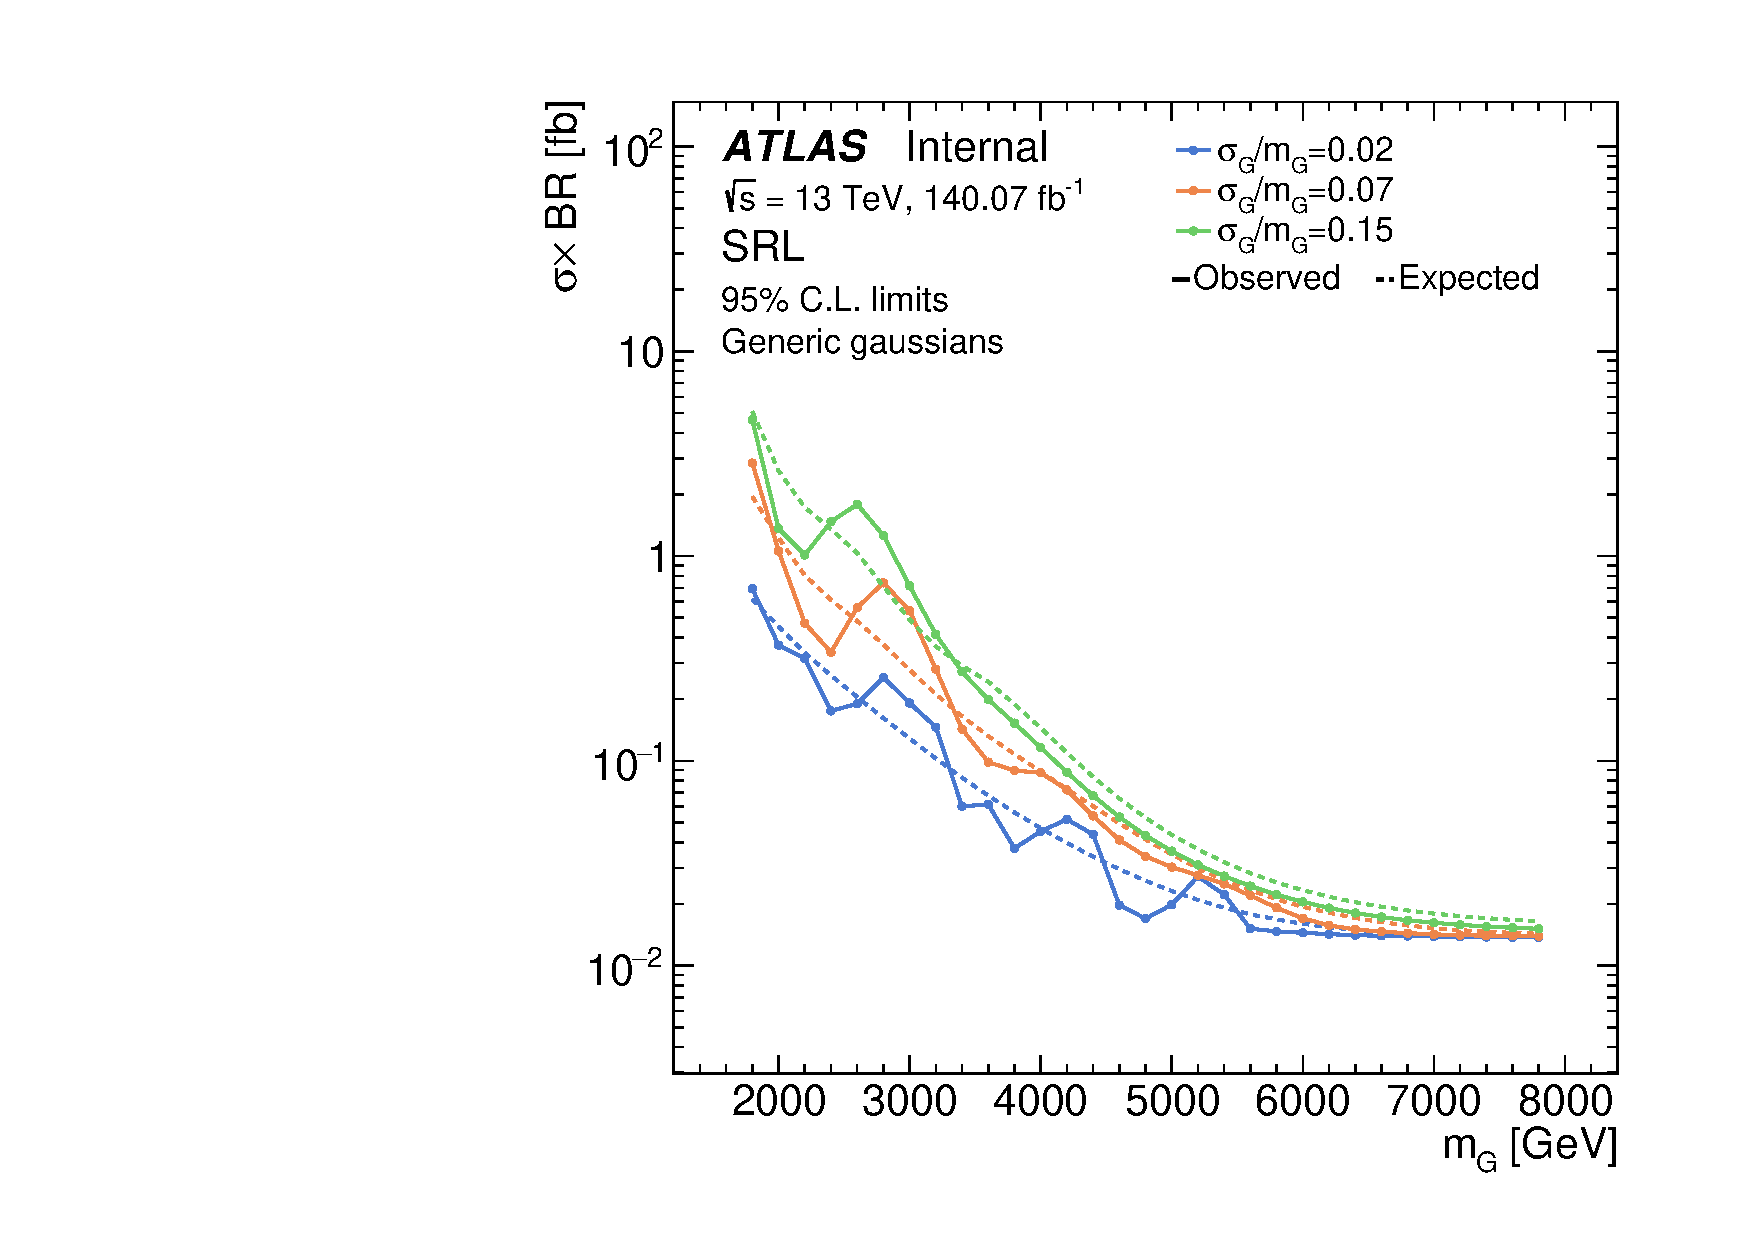
\includegraphics[width=\linewidth]{5_resonances/results/sigbkg/gaus/region/SRL50/can__gaus__SRL50____SRL50__gaus__width0p02_width0p07_width0p15__Run2}
        \caption{SRL.}
    \end{subfigure}
    \begin{subfigure}[h]{0.49\linewidth}
        \centering
        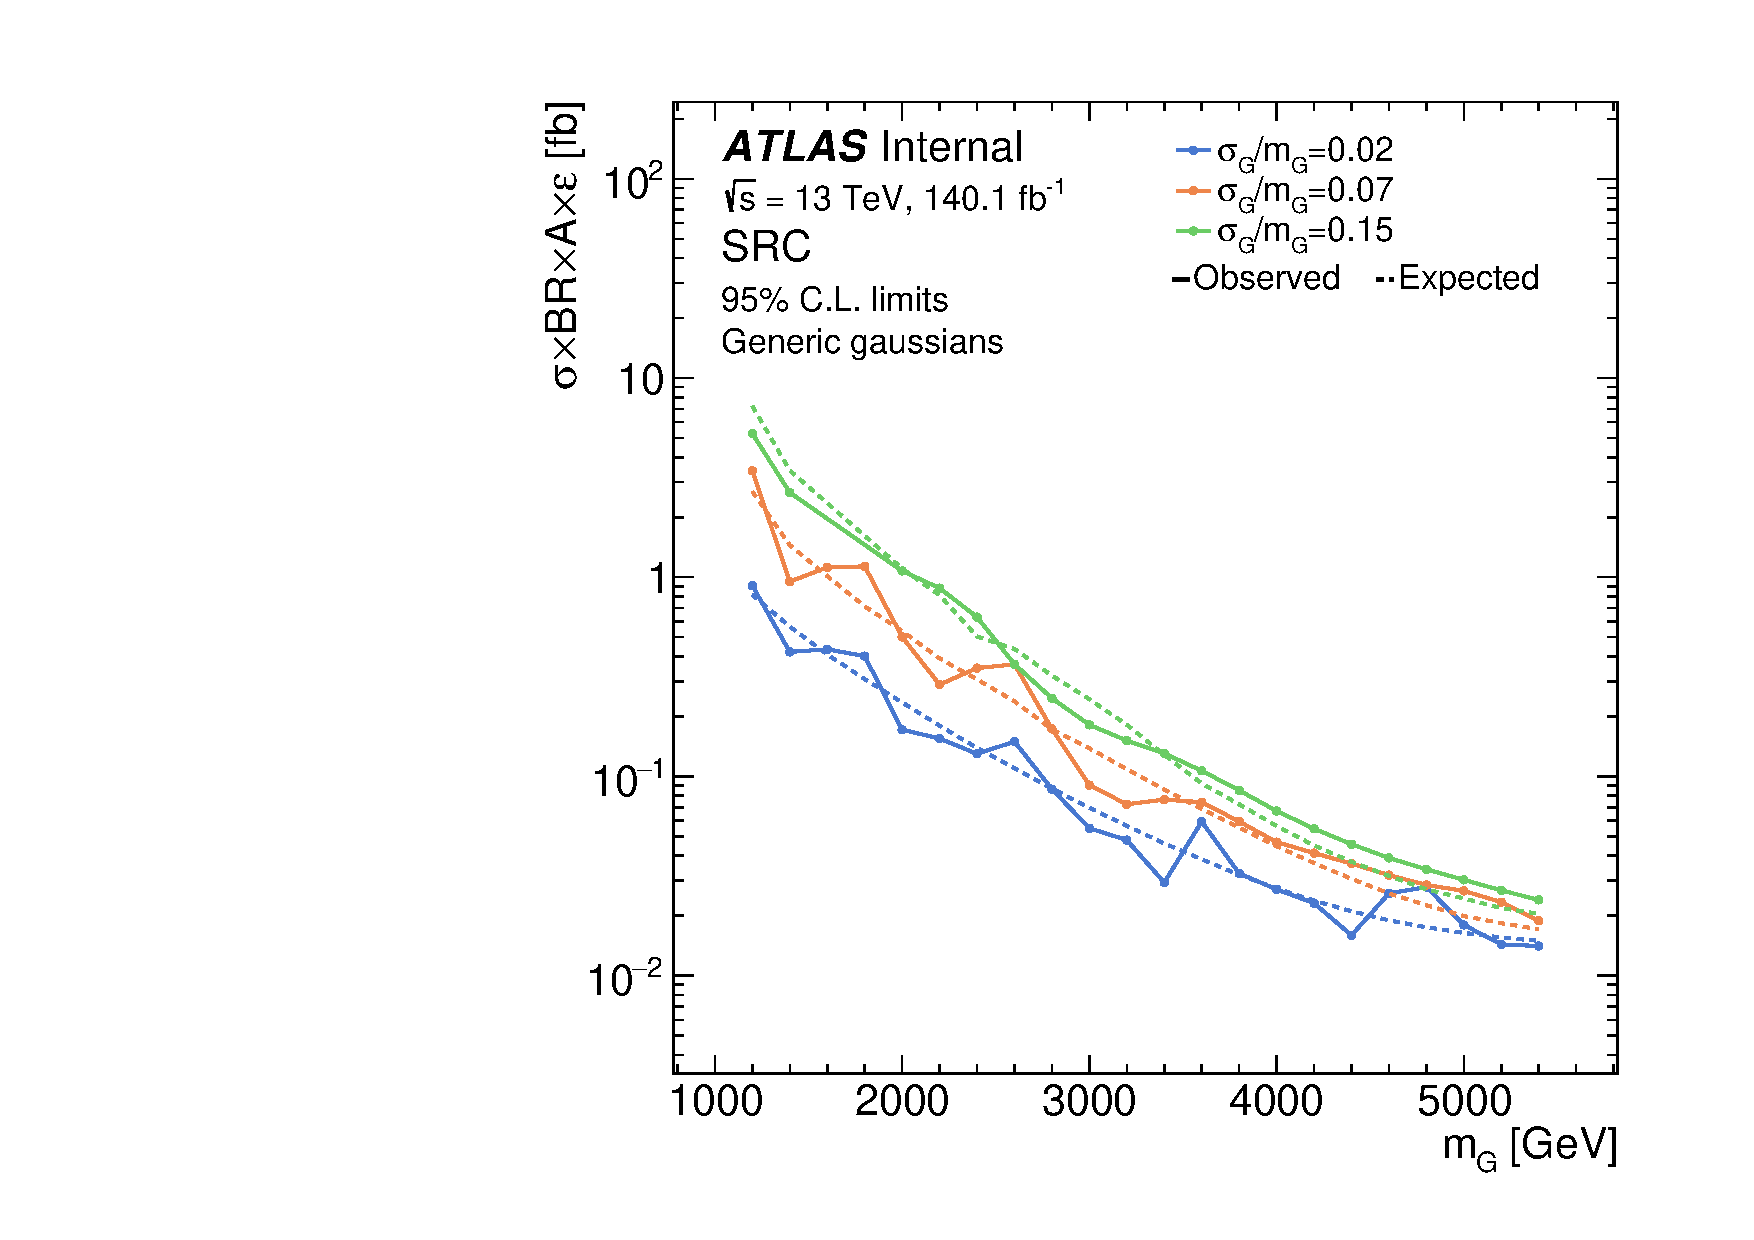
\includegraphics[width=\linewidth]{5_resonances/results/sigbkg/gaus/region/SRC50/can__gaus__SRC50____SRC50__gaus__width0p02_width0p07_width0p15__Run2}
        \caption{SRC.}
    \end{subfigure}
    \begin{subfigure}[h]{0.49\linewidth}
        \centering
        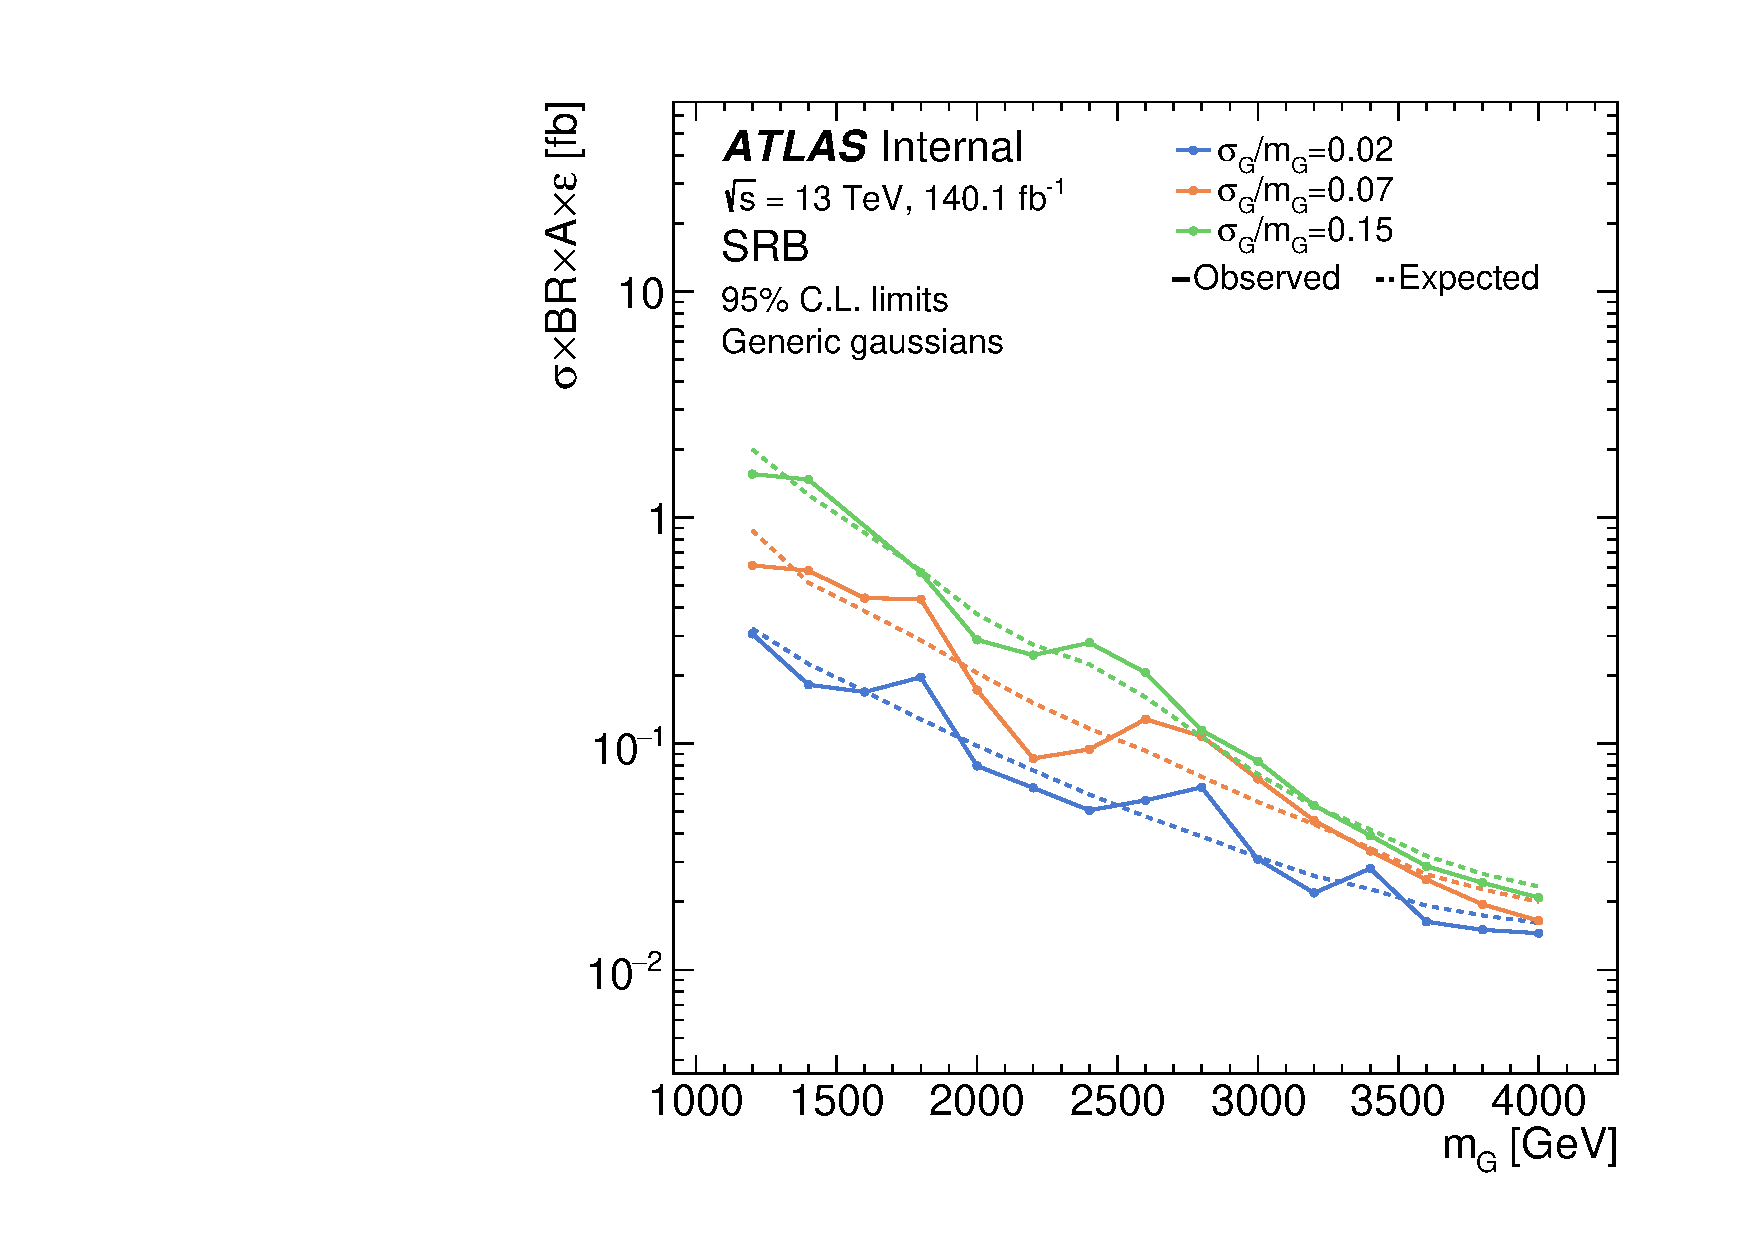
\includegraphics[width=\linewidth]{5_resonances/results/sigbkg/gaus/region/SRB/can__gaus__SRB____SRB__gaus__width0p02_width0p07_width0p15__Run2}
        \caption{SRB.}
    \end{subfigure}
    \caption{Límites observados y esperados en señales genéricas gaussianas con tres anchos diferentes: \(\sigma_G/m_G = 0.02, \, 0.07\) y \(0.15\); en las regiones SR, SRL, SRC y SRB.}
    \label{fig:results:results:bkgsig:results:gaus:limits}
\end{figure}

\begin{figure}[ht!]
    \centering
    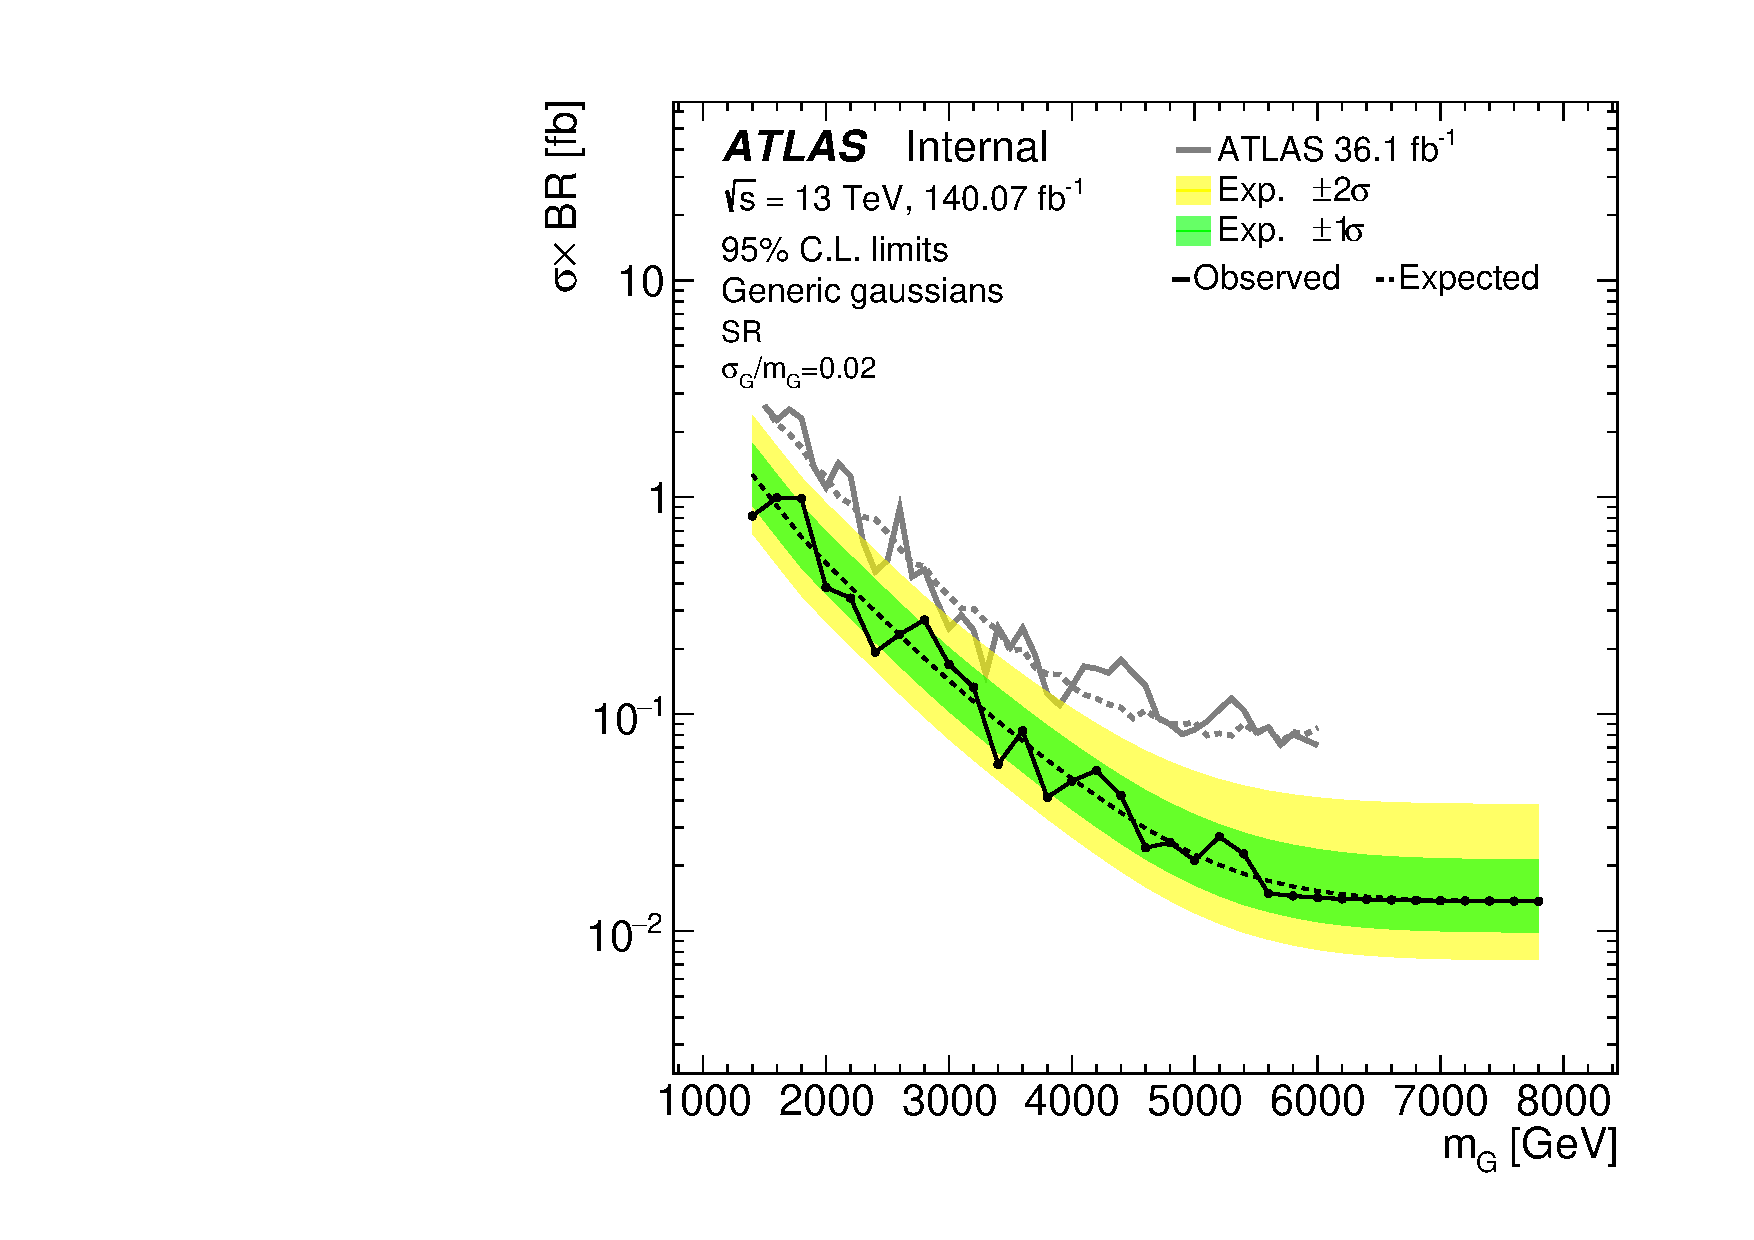
\includegraphics[width=0.6\linewidth]{5_resonances/results/sigbkg/gaus/fixed_param/width0p02/can__gaus__width0p02__width0p02____gaus__SR_oldexp_oldobs__Run2}
    \caption{Comparación de los límites observados y esperados en resonancias de forma Gaussiana con ancho del \(2\%\) obtenidos en este trabajo (líneas negras) con los de los resultados previos de \ac{ATLAS} utilizando datos recolectados en los años 2015-2016 (gris). Los límites esperados se muestran con las líneas punteadas mientras que los límites observados con las líneas sólidas.}
    \label{fig:results:results:bkgsig:results:gaus:limits_comparison_old}
\end{figure}


Por último, en la \Fig{\ref{fig:results:results:bkgsig:results:gaus:limits_comparison_old}}, se presenta una comparación de los resultados actuales con los últimos resultados de \ac{ATLAS} sobre resonancias gaussianas en el estado final de \gammajet. La búsqueda anterior se realizó utilizando únicamente el conjunto de datos de 2015+2016 recolectado por \ac{ATLAS}, con una luminosidad integrada total de \(36.1~\ifb\). Dado que el límite superior de la sección eficaz escala con la luminosidad como \(1 / \sqrt{L}\), cabría esperar una mejora de \(\sqrt{140.07} / \sqrt{36.1} \approx 1.96\) en el límite superior. Sin embargo, como se observa en las figuras, se obtiene una mejora mayor de la sensibilidad en el análisis actual, donde el límite superior en \(5500~\gev\) se mejora en un factor de aproximadamente 5.3. En consecuencia, con los resultados actuales, en virtud de un modelado de fondo más sofisticado, es posible aumentar las mejoras que se obtendrían utilizando sólo más datos en un factor de \(\sim 2.7\).